\chapter{Infrastructure and Environment for LLMOps}
\label{ch:infra}
\newrefsegment

% ----------------------------
% Chapter 3 — Abstract (online)
% ----------------------------
\abstract*{This chapter develops infrastructure as a first-class component of LLMOps. We begin with workload-driven hardware selection, contrasting GPU and TPU options across training, fine-tuning, and inference regimes, and we introduce practical cost models that relate throughput to cost per token under varying utilization. We then show how Infrastructure-as-Code (IaC) and environment standardization enable reproducibility, compliance, and low mean-time-to-recovery, emphasizing modular provisioning, policy-as-code, and secure secret management. Next, we cover containerization and Kubernetes orchestration for GPU fleets, including node labeling/taints, health probes, autoscaling patterns, and advanced scheduling strategies (e.g., multi-tenancy and partitioning). We survey modern serving stacks (e.g., optimized inference engines and batching/caching strategies) and discuss deployment topologies spanning cloud-native, hybrid, and multi-region architectures. The chapter concludes with an Ishtar AI infrastructure blueprint that ties these decisions to concrete operational outcomes—latency, throughput, reliability, and cost—supported by checklists intended for production deployment.}

\epigraph{\emph{``Without the right foundation, even the most advanced models will stumble.''}}{David Stroud}

% --- Reader-visible abstract (PDF) ---
\textbf{Abstract} This chapter develops infrastructure as a first-class component of LLMOps. We begin with workload-driven hardware selection, contrasting GPU and TPU options across training, fine-tuning, and inference regimes, and we introduce practical cost models that relate throughput to cost per token under varying utilization. We then show how Infrastructure-as-Code (IaC) and environment standardization enable reproducibility, compliance, and low mean-time-to-recovery, emphasizing modular provisioning, policy-as-code, and secure secret management. Next, we cover containerization and Kubernetes orchestration for GPU fleets, including node labeling/taints, health probes, autoscaling patterns, and advanced scheduling strategies (e.g., multi-tenancy and partitioning). We survey modern serving stacks (e.g., optimized inference engines and batching/caching strategies) and discuss deployment topologies spanning cloud-native, hybrid, and multi-region architectures. The chapter concludes with an Ishtar AI infrastructure blueprint that ties these decisions to concrete operational outcomes—latency, throughput, reliability, and cost—supported by checklists intended for production deployment.

\begin{tcolorbox}[
  title={\textbf{Chapter Overview}},
  colback=blue!5,
  colframe=blue!40!black,
  colbacktitle=blue!20,
  coltitle=black,
  fonttitle=\bfseries,
  boxrule=0.7pt,
  arc=4pt,
  left=5mm, right=5mm, top=4mm, bottom=4mm
]
\noindent\textbf{Chapter roadmap.}
This chapter develops the infrastructure layer as a first-class component of LLMOps:
\begin{itemize}[leftmargin=1.5em, itemsep=3pt]
    \item Workload-driven hardware selection (GPU/TPU and accelerator alternatives)
    \item Cost and capacity planning formalization
    \item Infrastructure-as-code patterns for reproducibility and compliance
    \item Containerization and Kubernetes-based orchestration for GPU fleets
    \item Serving-stack design (engines, scheduling, and memory management)
    \item Deployment patterns (cloud, hybrid, multi-region) and a concrete \ishtar{} implementation blueprint
\end{itemize}

\medskip
\noindent\textbf{Learning objectives.} After reading this chapter, you will be able to:
\begin{itemize}[leftmargin=1.5em, itemsep=3pt]
    \item Select and configure compute resources for LLM workloads
    \item Design resilient architectures with high availability
    \item Manage containerized deployments using Kubernetes
    \item Implement Infrastructure-as-Code for reproducibility
    \item Build secure, compliant systems with policy-as-code
\end{itemize}
\end{tcolorbox}

\section{Introduction}
\label{sec:ch3-introduction}

The infrastructure layer is the bedrock of any Large Language Model Operations (LLMOps) pipeline.
Without a carefully engineered environment, even state-of-the-art models will underperform, incur unnecessary costs, or introduce operational risks.
This chapter provides a comprehensive guide to designing, deploying, and managing the hardware, software, and network environments that power advanced LLM applications, illustrated through the lens of the \ishtar{} AI case study.
We dive into the practical realities of infrastructure for LLMOps—examining not only what each component does, but also why it matters, what trade-offs exist, and how decisions interact at scale.

Recent research underscores the convergence of LLMs and IaC, highlighting their combined potential to automate and streamline infrastructure provisioning.
LLMs are increasingly able to generate deployable IaC templates directly from natural language descriptions, thereby reducing the steep learning curve traditionally associated with infrastructure automation~\cite{garg2024infra-centric-iac,srivatsa2024-iac-llm}.
This informs our exploration of LLMOps infrastructure, positioning it not simply as a technical prerequisite but as a strategic enabler of scalability, cost-efficiency, and reliability—hinting at a future where LLMs may assist in managing their own infrastructure.

% ==================================================================
% ==================================================================
\section{Hardware Selection for LLM Workloads}\index{hardware!selection}
\label{sec:infra-hardware-bench}
Screenshot 2026-01-02 at 14.38.02
Selecting optimal hardware for LLM training and inference is a multi-dimensional decision involving performance, scalability, and cost considerations. 
An LLMOps practitioner must understand the differences between available accelerators, their architectural trade-offs, and the workload profiles for which they are best suited. 
Large Language Model workloads typically demand two primary hardware capabilities: (1) high-throughput matrix compute (for Transformer attention and feed-forward operations) and (2) large, high-bandwidth memory to store model weights and intermediate activations~\cite{nvidia-h100-arch,nvidia-a100-arch,jouppi2023-tpuv4}. 
This section examines the spectrum of hardware options—focusing on NVIDIA GPUs (L4, A100, H100) and Google TPUs (v4, v5e)—and analyzes their trade-offs for various LLM use cases (training, fine-tuning, and inference).

\subsection{Compute Profiles and Workload Types}
\label{sec:infra-hardware-profiles}

LLMs can stress hardware in different ways depending on the task. Training workloads are typically throughput-bound, benefiting from accelerators optimized for fast matrix multiplications and dense compute, whereas inference workloads often emphasize latency (time-to-first-token, TTFT) and memory capacity for serving multiple concurrent requests. Fine-tuning tasks (e.g., using parameter-efficient methods) fall somewhere in between.

To formalize these considerations, we decompose the latency $\ell$ of a single request into two components: time-to-first-token (TTFT) and time-per-output-token (TPOT). If $N_{\text{out}}$ is the number of output tokens, the total latency can be modeled as:
\begin{equation}
\ell = \ell_{\text{TTFT}} + N_{\text{out}} \cdot \ell_{\text{TPOT}} ~,
\label{eq:latency-infra}
\end{equation}
where $\ell_{\text{TTFT}}$ is largely determined by the initial forward pass over the input prompt (the prefill phase) and $\ell_{\text{TPOT}}$ is the incremental decoding latency per token in the autoregressive phase.

For batch processing of multiple requests, throughput becomes a key metric. If a batch of size $B$ completes in time $T_{\text{batch}}$, the system throughput is:
\begin{equation}
\Theta_{\text{req/s}} \approx \frac{B}{T_{\text{batch}}},
\qquad
\Theta_{\text{tok/s}} \approx \frac{B \cdot N_{\text{out}}}{T_{\text{batch}}} ~,
\label{eq:throughput-env}
\end{equation}
where $\Theta_{\text{req/s}}$ measures requests per second and $\Theta_{\text{tok/s}}$ tokens per second. Batching requests usually increases overall throughput $\Theta$ but can raise $\ell_{\text{TTFT}}$ due to queuing delays. Thus, optimal operating points depend on workload characteristics and service level agreements (SLAs). These SLAs function as \emph{operational contracts} that define latency budgets and throughput guarantees—contracts that infrastructure must deliver and that CI/CD pipelines (Chapter~\ref{ch:cicd}) and monitoring systems (Chapter~\ref{ch:monitoring}) must enforce. Some applications may prefer the lowest latency for each request (e.g., interactive chat), while others may trade a slight latency increase for dramatically higher throughput (e.g., batch summarization). The infrastructure choice determines which of these contracts can be honored.

Memory demands are another critical aspect. The attention key-value (KV) cache grows linearly with sequence length and batch size. For a decoder-only Transformer with $L$ layers and $H$ attention heads of dimension $d_h$, the approximate memory required is:
\begin{equation}
M_{\text{KV}} \approx 2 \cdot L \cdot B \cdot H \cdot d_h \cdot T \cdot \alpha ~,
\label{eq:kv-memory}
\end{equation}
where $T$ is the sequence length and $\alpha$ the bytes per element (e.g., 2 for FP16, 1 for INT8). The factor 2 accounts for storing both keys and values. 

This linear dependence means that long-context or high-concurrency serving can easily become memory-bound. For example, a single 13B-parameter model (like LLaMA-13B with 40 layers and 40 heads of dimension 128) will require on the order of 1–2 GB of GPU memory per 1024 tokens of context \textit{per request} in FP16 precision.\footnote{Empirical estimates from practitioner reports indicate $\sim$10–15 GB just for KV caches when serving a batch of eight concurrent requests at 1024-token contexts.} Caching and memory management strategies (see \S\ref{sec:infra-hardware-bench}) are therefore central to efficient operations.

\subsection{GPU Architectures and Choices}\index{GPU!architecture}
\label{sec:infra-hardware-gpu}

NVIDIA GPUs remain the dominant hardware for LLM workloads in 2024–2025. The NVIDIA L4 offers excellent per-watt efficiency for smaller models, embeddings, and lightweight inference; the A100 was the mainstream workhorse for both training and inference in the early 2020s; and the H100 (Hopper architecture) introduces new low-precision math (FP8), significantly higher memory bandwidth, and other architectural improvements targeting Transformer models. 

\begin{table}[t]
  \centering
  \caption{GPU accelerator selection determines cost, throughput, and deployment feasibility. Different accelerators optimize for different model sizes and workloads: A100 provides balanced performance, H100 offers higher throughput and FP8 support, L4 enables cost-effective smaller models. Choose based on model size, traffic volume, and budget constraints.}
  \label{tab:ch03_gpucompare}
  \begin{tabular}{lcccc}
    \hline
    Processor & Memory & Tokens/s (13B) & Price/hr (cloud) & Best Use Case \\
    \hline
    NVIDIA L4     & 24 GB & $\sim$2{,}000 & \$0.35 & Low-power, low-latency inference; embeddings \\
    NVIDIA A100   & 40 GB & $\sim$6{,}500 & \$2.90 & High-load inference; some training/fine-tuning \\
    NVIDIA A100   & 80 GB & $\sim$8{,}000 & \$3.80 & Larger models; multi-model serving \\
    NVIDIA H100   & 80 GB & $\sim$12{,}000 & \$5.00 & Cutting-edge throughput; FP8 acceleration \\
    \hline
  \end{tabular}
\end{table}

The H100 generally outperforms the A100 across both training and inference, thanks to innovations like fourth-generation Tensor Cores with the Transformer Engine (enabling FP8 precision) and much higher HBM3 memory bandwidth (3.35~TB/s vs. 2.0~TB/s on A100)~\cite{nvidia-h100-arch,nvidia-a100-arch}. In practice, for LLMs in the 13B–70B parameter range, an A100-80GB can deliver about 130 tokens/s, while an H100 can reach 250–300 tokens/s under similar conditions. This translates into significantly lower cost-per-token for inference. Independent benchmarks show the H100 achieving nearly 2$\times$ the throughput of an A100 at the same batch size and faster TTFT for a 7B model using optimized inference libraries~\cite{tgi-github,vllm-pagedattention}. 

The A100 remains widely available and is still highly capable. Its 80 GB variant is valuable for long-context inference or hosting multiple models simultaneously (where memory capacity is critical). Meanwhile, the smaller NVIDIA L4 (24 GB) offers superb efficiency for less demanding tasks: running quantized 7B–13B models for embeddings or classification, or servicing low-latency interactive jobs where throughput needs are moderate. In heterogeneous fleets, L4s excel at ``small jobs'' with an attractive cost and power profile.

\subsection{TPU Architectures and Considerations}\index{TPU!architecture}
\label{sec:infra-hardware-tpu}


In cloud settings, purpose-built accelerators such as AWS Trainium2/Inferentia2 introduce a parallel serving ecosystem (AWS Neuron), requiring separate kernel/toolchain considerations but offering attractive price/performance profiles for certain inference and training regimes~\cite{aws_trainium2_arch,aws_inferentia_overview,aws_neuron_arch_guide}.
Google’s Tensor Processing Units (TPUs) provide an alternative accelerator optimized for large-scale matrix multiplications. The TPU v4, widely used internally at Google and now available on Google Cloud, provides 32 GB HBM per chip and is typically deployed in multi-chip pods (8–256 chips). TPUs shine in training workloads due to their high FLOPs per dollar and fast interconnect bandwidth, but are increasingly used for inference as well. They favor bfloat16 (BF16) and INT8 formats (analogous to GPUs’ FP16/FP8) for efficiency~\cite{jouppi2023-tpuv4}. While a single TPU v4 chip has less memory than a high-end GPU (32 GB vs 80 GB), TPU pods can scale out with near-linear efficiency on large workloads. 

In batch-heavy deployments (e.g., serving many requests in parallel), TPU v4 pods can reduce cost-per-token by an estimated 20–30\% compared to GPU clusters. Their drawbacks are ecosystem maturity (PyTorch support is still catching up to JAX/TF) and availability (primarily limited to Google Cloud). Newer TPUs like the TPU v5e (announced 2024) are explicitly aimed at inference with a focus on throughput per dollar. Google reports that TPU v5e offers a 2.3$\times$ price-performance improvement over TPU v4 for LLM training, and early results show inference efficiency gains as well (e.g., continuous batching and sliding window attention via JetStream). In one reported example, a TPU v5e-8 (8 chips) achieved $\sim$4{,}783 tokens/s serving a LLaMA-2 7B model with INT8 quantization—roughly on par with a cluster of 4–8 high-end GPUs but at lower cost.

% ==================================================================
\section{Cost Modeling and Economics}\index{cost!modeling}
\label{sec:infra-cost}

Building and operating LLM infrastructure at scale brings significant costs. In this section, we dive deeper into modeling those costs and techniques to optimize them. We cover the economics of token generation, the impact of batch size on utilization, and how caching and quantization influence cost.

\subsection{Token Economics and Cost per Query}
\label{sec:infra-cost-tokens}

A key metric in LLMOps is the cost per generated token (or per thousand tokens)---essentially, how many dollars does it take in GPU/TPU time to produce the model’s output. As introduced earlier (Equation~\ref{eq:costptok}), this depends on hardware cost and throughput. It is also useful to break cost down per request, especially if the system has a mix of prompt lengths and completion lengths. 

If an average request in an application is $N_{\text{in}}$ input tokens and $N_{\text{out}}$ output tokens, then the computation required will be roughly proportional to:
\[
N_{\text{in}} \times L \; + \; N_{\text{out}} \times L , \label{eq:costptok}
\]
where $L$ is the number of Transformer layers, and noting that each output token also involves attention over all prior tokens. Thus longer prompts or longer outputs linearly increase compute and latency, which linearly increases cost. This is why many LLM API providers charge separately for input tokens vs.\ output tokens—they both consume cycles.

From an infrastructure owner's perspective, tracking cost per 1k tokens is very useful. Table~\ref{tab:ch03_cost_per_token} illustrates this with concrete examples comparing GPU options under different utilization scenarios.

\begin{table}[t]
  \centering
  \caption{Cost per token varies significantly with utilization and hardware choice. Higher utilization amortizes fixed costs, making H100 cost-effective at scale despite higher hourly rates. Choose A100 for variable workloads with low average utilization; choose H100 for sustained high-throughput deployments where utilization exceeds 60\%.}
  \label{tab:ch03_cost_per_token}
  \small
  \setlength{\tabcolsep}{10pt}
  \renewcommand{\arraystretch}{1.4}
  \begin{tabularx}{\linewidth}{@{}lccX@{}}
    \toprule
    \rowcolor{blue!15}
    \textbf{GPU Type} & \textbf{Utilization} & \textbf{Cost/hr} & \textbf{Cost per 1k tokens} \\
    \midrule
    \rowcolor{blue!8}
    A100 (80GB) & \textcolor{green!70!black}{\textbf{100\%}} & \$3.80 & \textcolor{blue!70!black}{\textbf{\$0.06}} \\
    & & & \footnotesize (8,000 tokens/sec) \\
    \addlinespace[2pt]
    \rowcolor{orange!12}
    A100 (80GB) & \textcolor{orange!70!black}{\textbf{50\%}} & \$3.80 & \textcolor{red!70!black}{\textbf{\$0.12}} \\
    & & & \footnotesize (4,000 tokens/sec effective) \\
    \addlinespace[2pt]
    \rowcolor{green!10}
    H100 (80GB) & \textcolor{green!70!black}{\textbf{100\%}} & \$5.00 & \textcolor{green!70!black}{\textbf{\$0.035}} \\
    & & & \footnotesize (12,000 tokens/sec) \\
    \bottomrule
  \end{tabularx}
  \vspace{3pt}
  \footnotesize
  \textit{Note:} The H100 at full utilization achieves nearly half the cost per token compared to an underutilized A100, demonstrating the importance of both hardware selection and utilization optimization~\cite{fabricated-knowledge-costs,lambda-gpt3-cost}.
\end{table}

The calculations show that a single A100 at \$3.80/hour generating 8,000 tokens/sec costs about \$0.47 per second, yielding $\sim$\$0.06 per thousand tokens at full utilization. However, if that same A100 only runs at 50\% utilization, the effective cost doubles to $\sim$\$0.12 per thousand tokens. By comparison, a newer H100 at \$5.00/hour generating 12,000 tokens/sec (under optimized settings) costs \$0.416 per second, i.e.\ $\sim$\$0.035 per thousand tokens---nearly half the cost of the underutilized A100~\cite{fabricated-knowledge-costs,lambda-gpt3-cost}. 

This simple math underscores two things: (1) newer hardware can indeed reduce marginal costs if fully utilized, and (2) utilization (keeping devices busy) is critical. Paying for an expensive GPU that is idle half the time is wasteful. Solutions such as auto-scaling and multi-tenancy are aimed precisely at keeping utilization high. Critically, these cost models become \emph{operational constraints} that define the economic boundaries within which the system must operate. These constraints form part of the operational contract: if infrastructure costs exceed budget thresholds, scaling strategies (Chapter~\ref{ch:scaling}) must respond by throttling or cost-aware capacity management.

\begin{quote}
\textit{Example.} Google Cloud reports that advanced infrastructure and optimized inference runtimes (e.g., JetStream on TPU v5e) can bring generation costs down to \$0.25–\$0.30 per million tokens, or $\sim$0.00025 per token~\cite{jouppi2023-tpuv4}.
\end{quote}

\begin{tcolorbox}[
  title={\textbf{Cost Modeling Example: Comparing GPU Options}},
  colback=orange!5,
  colframe=orange!40!black,
  colbacktitle=orange!20,
  coltitle=black,
  fonttitle=\bfseries,
  boxrule=0.7pt,
  arc=4pt,
  left=5mm, right=5mm, top=4mm, bottom=4mm,
  before skip=6pt,
  after skip=6pt
]
In practice, cost modeling often involves simulating different deployment scenarios. For example, if you expect \textbf{100 requests per second} each generating \textbf{200 tokens}, that is \textbf{20k tokens/sec throughput} needed. How many GPUs of type X are required to sustain that?

\begin{itemize}[leftmargin=1.5em, itemsep=4pt]
    \item \textbf{Option 1: A100 GPUs} — If each A100 can do $\sim$8k/sec, you would need \textbf{3 A100s} (at \$3.80/hr each, so \textbf{\$11.4/hr}).
    \item \textbf{Option 2: H100 GPUs} — Maybe \textbf{2 H100s} could do it (2 $\times$ \$5.00 = \textbf{\$10/hr}), slightly cheaper.
    \item \textbf{Option 3: L4 GPUs} — Or perhaps \textbf{5 L4 GPUs} (5 $\times$ \$0.35 = \textbf{\$1.75/hr}), but at $\sim$2k/sec each, 5 L4s only yield \textbf{10k/sec}---not enough.
\end{itemize}

This back-of-the-envelope calculation shows that while L4s are cheap, you would need too many of them in this scenario. On the other hand, if the workload was lighter (say \textbf{2k tokens/sec}), a single A100 would be overkill and an L4 could handle it at \textbf{one-eighth the hourly cost}.
\end{tcolorbox}

Thus, rightsizing hardware to workload is important---and in many cases a mix of different instance types (as Ishtar uses) is the optimal solution.

\subsection{Batch Size vs Throughput Trade-offs}
\label{sec:infra-cost-batch}

As discussed earlier, increasing the batch size $B$ (number of requests processed together) can greatly improve hardware efficiency and throughput $\Theta$, up to a point. The diminishing returns occur when the device is fully busy and additional requests mainly add waiting time. It is useful to actually measure throughput vs.\ batch size on your model. Often, the first few requests amortize overhead (so going from batch 1 to 4 might yield a 3$\times$ throughput gain), but beyond a certain batch (say 32) each increment yields a smaller gain. In some cases, throughput even saturates---e.g., batch 64 and 128 might achieve the same tokens/sec---because some other bottleneck (memory or kernel launch overhead) has been hit~\cite{tgi-github,tgi_docs}. 

Crucially, batch size affects latency for each request. In a naïve batching system, an incoming request might wait until enough other requests arrive to form a batch of size $B_{\text{target}}$. This waiting adds to TTFT (queuing delay). If requests arrive very frequently, this delay is negligible (the batch fills in a few milliseconds). But if traffic is bursty or low, forcing a large batch can hurt latency. 

Modern inference servers implement dynamic batching to mitigate this: rather than a fixed batch, they batch whatever requests have arrived within a small time window (e.g., 10–50 ms). This ensures some batching even in irregular traffic, without indefinite waits. Adaptive batching algorithms further adjust the window based on recent load to hit a performance goal.

From a cost perspective, batching is one of the biggest levers to reduce cost per output. Running a single request at a time on a GPU leaves much of the GPU’s parallelism underutilized (especially during the autoregressive phase when each token is generated sequentially per request). By batching many requests, the GPU can do matrix multiplies for many tokens at once, reaching high occupancy. Reports show that enabling continuous batching in production LLM APIs dramatically increased throughput with only slight added latency~\cite{tgi-github,tgi_docs}. The flip side is that you must have concurrent load to take advantage of it. If your app only serves one user at a time, you cannot magically batch their requests (though speculative decoding is a related technique we will revisit later).

In summary, it is best to operate GPUs at a batch size that still meets your latency SLA. If latency is more critical, you may run at small batches and accept higher cost per token. If throughput (and cost) is key, you batch aggressively and perhaps even do asynchronous processing (queue up work and process in big chunks). Interactive services often find a middle ground: small batches during off-peak (to keep latency low) and larger batches during peak (trading a bit more latency for major throughput gain when many users are active).

\begin{figure}[t]
  \centering
  \begin{llmfigbox}
  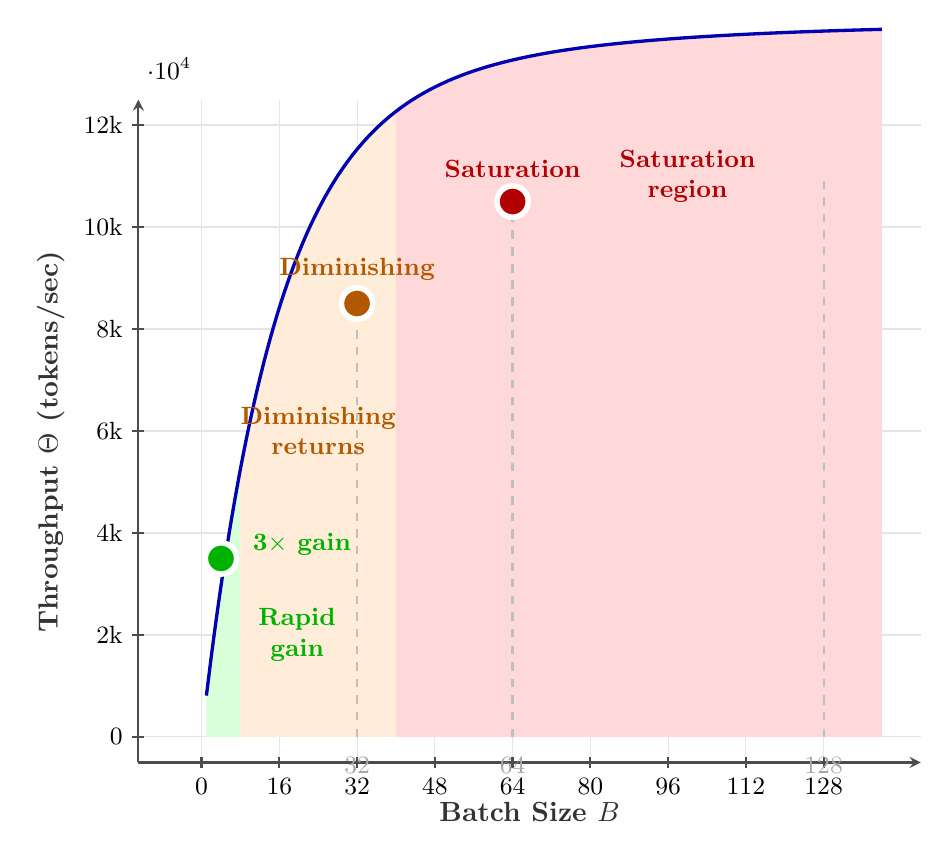
\begin{tikzpicture}[font=\small]
    \begin{axis}[
      width=0.95\textwidth,
      height=10cm,
      xlabel={Batch Size $B$},
      ylabel={Throughput $\Theta$ (tokens/sec)},
      xmin=-5, xmax=140,
      ymin=0, ymax=12000,
      grid=major,
      grid style={gray!20},
      axis lines=left,
      axis line style={thick, color=black!70},
      tick style={thick, color=black!70},
      xlabel style={font=\normalsize\bfseries, color=black!80, yshift=4pt},
      ylabel style={font=\normalsize\bfseries, color=black!80, xshift=-4pt},
      xtick={0,16,32,48,64,80,96,112,128},
      ytick={0,2000,4000,6000,8000,10000,12000},
      yticklabels={0,2k,4k,6k,8k,10k,12k},
      tick label style={font=\small},
      every axis plot/.append style={smooth},
      clip=false,
      enlarge x limits={abs=8},
      enlarge y limits={abs=500}
    ]
      
      % Define the throughput function (diminishing returns curve)
      \pgfmathdeclarefunction{throughput}{1}{%
        \pgfmathparse{12000 * (1 - exp(-#1/15)) + 2000 * (1 - exp(-#1/50))}%
      }
      
      % Add shaded regions for different phases (behind the curve)
      \addplot[
        fill=green!15,
        draw=none,
        domain=1:8,
        area legend
      ] {throughput(x)} \closedcycle;
      
      \addplot[
        fill=orange!15,
        draw=none,
        domain=8:40,
        area legend
      ] {throughput(x)} \closedcycle;
      
      \addplot[
        fill=red!15,
        draw=none,
        domain=40:140,
        area legend
      ] {throughput(x)} \closedcycle;
      
      % Main throughput curve (diminishing returns) - thick blue line
      \addplot[
        very thick,
        color=blue!70!black,
        smooth,
        domain=1:140,
        samples=150
      ] {throughput(x)};
      
      % Add reference lines at key batch sizes (32, 64, 128)
      \addplot[dashed, color=gray!50, thick, line width=0.8pt] coordinates {(32,0) (32,8500)};
      \addplot[dashed, color=gray!50, thick, line width=0.8pt] coordinates {(64,0) (64,10500)};
      \addplot[dashed, color=gray!50, thick, line width=0.8pt] coordinates {(128,0) (128,11000)};
      
      % Annotate key points with colored markers
      \node[circle, fill=green!70!black, draw=white, line width=2pt, inner sep=4pt] at (axis cs:4,3500) {};
      \node[font=\small\bfseries, text=green!70!black, above=5pt, right=8pt] at (axis cs:4,3500) {3$\times$ gain};
      
      \node[circle, fill=orange!70!black, draw=white, line width=2pt, inner sep=4pt] at (axis cs:32,8500) {};
      \node[font=\small\bfseries, text=orange!70!black, above=5pt] at (axis cs:32,8500) {Diminishing};
      
      \node[circle, fill=red!70!black, draw=white, line width=2pt, inner sep=4pt] at (axis cs:64,10500) {};
      \node[font=\small\bfseries, text=red!70!black, above=5pt] at (axis cs:64,10500) {Saturation};
      
      % Add phase labels in shaded regions (larger font for readability, positioned to be visible)
      \node[font=\small\bfseries, text=green!70!black, align=center, right=10pt] at (axis cs:4,2000) {Rapid\\gain};
      \node[font=\small\bfseries, text=orange!70!black, align=center] at (axis cs:24,6000) {Diminishing\\returns};
      \node[font=\small\bfseries, text=red!70!black, align=center] at (axis cs:100,11000) {Saturation\\region};
      
      % Add batch size labels on x-axis for key points
      \node[font=\small, text=gray!70, below=4pt] at (axis cs:32,0) {32};
      \node[font=\small, text=gray!70, below=4pt] at (axis cs:64,0) {64};
      \node[font=\small, text=gray!70, below=4pt] at (axis cs:128,0) {128};
      
    \end{axis}
  \end{tikzpicture}
  \end{llmfigbox}
  \caption{Throughput vs.\ batch size trade-off determines capacity planning and latency SLOs. Increasing batch size initially yields large throughput gains (e.g., 3$\times$ improvement from batch 1 to 4), but returns diminish beyond batch size 32. Eventually throughput saturates (batch 64 and 128 achieve similar tokens/sec) as memory or kernel launch overhead becomes the bottleneck. Understanding this saturation point helps teams optimize batch sizes for their latency requirements and hardware constraints.}
  \label{fig:ch03_batchtradeoff}
\end{figure}

\subsection{Caching and Quantization Effects}
\label{sec:infra-cost-quant}

Beyond raw compute, two techniques significantly impact performance and cost in LLM serving: caching and quantization.

\subsubsection{KV Cache and Prompt Caching} 
Transformers benefit from caching past key/value tensors so that each new token does not recompute attention for all previous tokens. Using the KV cache yields huge speedups for long sequences---after the first token, each subsequent token’s attention is only over the latest token vs.\ all previous. However, the KV cache consumes a lot of memory (growing with sequence length). In practice, this means that serving long prompts or generating long outputs can memory-bind GPUs, limiting batch size or requiring high-memory GPUs. For example, LLaMA-2 13B was reported to use on the order of $\sim$1 MB of VRAM per generated token (in FP16) for the KV cache---so a 4k-token generation uses $\sim$4 GB for one request. This is comparable to the model weights themselves in size.

As a result, many innovations in 2024–2025 have targeted KV cache optimization. One approach is KV compression or dropping: techniques like \emph{SnapKV} (2024) select only the “important” past tokens to keep in cache for each head, discarding others, which yielded up to 3.6$\times$ faster generation and 8.2$\times$ lower memory use on 16k sequences with negligible accuracy loss. Others like \emph{AQUA-KV} dynamically quantize the KV tensors to lower precision on the fly, shrinking memory footprint adaptively. Yet others use paging of the KV to CPU memory or disk when not in active use (e.g., the vLLM library’s \emph{PagedAttention})~\cite{vllm-pagedattention,pagedattention_paper}. The net effect is to allow either longer contexts on the same GPU or more concurrent requests, which improves throughput and cost efficiency. In fact, vLLM’s paging strategy can improve effective throughput dramatically by avoiding wasted padding in naïve batch implementations---one report showed up to 24$\times$ higher throughput than naïve batching in certain workloads~\cite{vllm-pagedattention,pagedattention_paper}.

\subsubsection{Quantization} 
Quantizing model weights (and even activations) from 16-bit to 8-bit or 4-bit is another powerful method to reduce cost. By using lower precision, models use less memory and run faster (since GPUs/TPUs can process more low-precision ops in parallel). 8-bit inference of large models is now common, with minimal accuracy loss, and can nearly double throughput vs.\ FP16. New H100 GPUs even support direct FP8 math to further accelerate this. Quantization directly translates to cost savings: if you can run the same workload on half the number of GPUs by using INT8 instead of FP16, you have nearly halved your cost. 

Google’s Cloud TPU team reported that with INT8 quantization for weights, activations, and KV cache, their JetStream engine achieved 3$\times$ more inferences per dollar compared to the previous baseline~\cite{jouppi2023-tpuv4}. Similarly, NVIDIA’s TensorRT can leverage INT8 for supported models to improve throughput by 2–4$\times$ (with calibration for minimal accuracy impact)~\cite{tensorrtllm-github,tensorrtllm_docs}. Not all models quantize equally well---some may require fine-tuning or calibration to retain accuracy at 4-bit. But the field has progressed such that many open models (e.g., LLaMA-2, GPT-J) have 4-bit and 8-bit versions available with negligible quality difference on many tasks. 

\subsubsection{Ishtar Case} 
After initial deployment, Ishtar quantized its 70B model to 8-bit, which improved throughput by $\sim$1.8$\times$ and cut the GPU fleet requirement by almost half, with only a minor quality drop on outputs. It also implemented a custom KV cache eviction policy to allow eight concurrent 2k-token requests on each A100 without out-of-memory errors, where previously it only ran four.

In sum, caching and quantization techniques both serve to get more out of hardware---either by reducing redundant computation (caching) or by packing more compute into the same memory/compute budget (quantization). An LLMOps infrastructure should be designed to take advantage of these, for instance by choosing inference frameworks that support quantized models and efficient KV caching.

\subsection{Worked Example: Cost per Million Tokens Across Accelerators}

To make the abstract formulas more tangible, Table~\ref{tab:ch03_costcompare} provides a back-of-the-envelope comparison of cost per million tokens across common accelerators. 
We assume on-demand cloud pricing (as of early 2025) and sustained throughput figures taken from public benchmarks and vendor reports. 
The effective cost per million tokens is calculated using Equation~\ref{eq:costptok}. 

\begin{table}[t]
  \centering
  \caption{Cost per token varies significantly across accelerators and utilization levels. Lower-cost accelerators (L4) become cost-effective for smaller models or variable workloads, while high-end accelerators (H100) justify their premium at high utilization with large models. When cost differences exceed 2$\times$, hardware choice becomes a primary cost optimization lever. Assumes typical sustained throughput for a 13B--70B model and on-demand cloud pricing.}
  \label{tab:ch03_costcompare}
  \begin{tabular}{lccc}
    \hline
    Accelerator & Hourly Price (\$) & Sustained Throughput (tok/s) & Cost per 1M tokens (\$) \\
    \hline
    NVIDIA A100-80GB & 3.80 & 8,000 & $\sim$0.13 \\
    NVIDIA H100-80GB & 5.00 & 12,000 & $\sim$0.09 \\
    Google TPU v4     & 3.00 & 9,000  & $\sim$0.093 \\
    Google TPU v5e-8  & 8.00\footnote{Eight TPU v5e chips at $\sim$\$1/hr each, deployed as a pod.} & 48,000 & $\sim$0.046 \\
    \hline
  \end{tabular}
\end{table}

Several insights emerge:
\begin{itemize}
    \item \textbf{H100 efficiency.} Despite a higher hourly cost, the H100’s greater throughput yields $\sim$30–40\% lower cost per token than the A100~\cite{nvidia-h100-arch}.
    \item \textbf{TPU v5e advantage.} The TPU v5e, designed for inference, achieves the lowest cost per million tokens in this comparison, owing to architectural efficiency and Google’s optimized JetStream runtime~\cite{jouppi2023-tpuv4}.
    \item \textbf{Utilization effect.} These numbers assume near-saturation throughput. If utilization drops (e.g., GPUs idle during off-peak hours), the effective cost rises proportionally. In real-world deployments, auto-scaling and multi-tenancy are essential to keep utilization high. This utilization requirement becomes an operational contract: infrastructure must maintain minimum utilization thresholds, and scaling systems (Chapter~\ref{ch:scaling}) must enforce these thresholds through intelligent capacity management.
\end{itemize}

This worked example shows that raw hourly prices can be misleading. A seemingly more expensive accelerator (H100) may deliver better economics than a cheaper one (A100) when measured in cost-per-output, and specialized hardware (TPU v5e) can further reduce unit costs in high-throughput scenarios.


% ==================================================================
\section{Infrastructure-as-Code (IaC) for LLMOps}\index{Infrastructure-as-Code}
\label{sec:iac}

Automating and codifying infrastructure is essential for reliability and scalability. 
Infrastructure-as-Code (IaC) refers to writing declarative or programmatic definitions for compute, networking, and software setup so that environments can be reproduced and managed consistently. 
In the context of LLMOps, where we may operate dozens of GPU nodes, specialized drivers, networking rules for data, and frequent changes during experimentation, IaC is a foundational requirement rather than a luxury~\cite{terraform-docs,pulumi-docs}.

\subsection{Why IaC Matters}
\label{sec:iac-why}

Without IaC, managing infrastructure often devolves into a series of manual steps (e.g., clicking in cloud consoles or running ad-hoc scripts) that are error-prone and hard to track. 
IaC addresses this by treating infrastructure the same way as application code---with version control, reviews, testing, and continuous deployment. 
Some key benefits include:

\begin{itemize}
  \item \textbf{Reproducibility and Consistency.} 
  IaC ensures every environment (development, staging, production) can be made identical by applying the same code. 
  This eliminates the ``works on my machine'' problem and prevents configuration drift over time~\cite{terraform-docs}. 
  For example, an exact clone of the production LLM serving stack can be spun up in a test environment to debug an issue.

  \item \textbf{Speed and Efficiency.} 
  Provisioning and updating infrastructure through code is much faster than manual operations. 
  Spinning up ten GPU machines with all required software can be done in minutes with an automated script versus hours or days manually. 
  This accelerates experimentation and scaling.

  \item \textbf{Version Control and Auditability.} 
  Infrastructure code in Git provides a history of changes---who changed what, when. 
  Rollbacks are as simple as reverting to an earlier commit. 
  During a compliance audit, code and change logs serve as evidence of controls~\cite{terraform-docs}. 
  Every change goes through code review, catching mistakes before they hit production.

  \item \textbf{Reduced MTTR (Mean Time to Recovery).} 
  If an environment breaks, IaC allows rapid recreation from scratch. 
  Disaster recovery is improved: if a whole region goes down, an LLM cluster can be redeployed in another region using the same code. 
  This ability to ``rebuild from code'' greatly reduces downtime in worst-case scenarios~\cite{opa-docs}.

  \item \textbf{Compliance and Security Automation.} 
  IaC makes it easier to enforce security rules globally. 
  For instance, if policy mandates that all storage buckets must be encrypted and non-public, this can be encoded into templates. 
  Policy-as-code frameworks (e.g., HashiCorp Sentinel, Open Policy Agent) validate IaC against security policies before deployment~\cite{sentinel-docs,opa-docs}. 
  Secrets (API keys, DB passwords) can be injected via secure stores rather than hard-coded, ensuring organizational guardrails are baked into both the code and the pipeline.

  \item \textbf{Documentation as Code.} 
  Infrastructure code itself becomes living documentation. 
  Instead of stale wikis, new engineers can read Terraform, Pulumi, or Helm files and understand the architecture. 
  This is crucial in complex LLMOps setups where one might ask: ``how many GPUs are in cluster X and what type are they?''---the code contains the answer.
\end{itemize}

In summary, IaC brings discipline and best practices from software engineering into operations. 
For LLMOps, where infrastructure can be complex (mix of GPU types, specialized networking, etc.) and stakes are high (a mistake can be very expensive), IaC is foundational for doing things reliably at scale~\cite{srivatsa2024-iac-llm}.

\subsection{Tooling Comparison}
\label{sec:iac-tools}


Terraform remains a dominant choice for declarative infrastructure provisioning, especially when paired with a module-based design system and collaborative workflows that enforce reviews and policy checks~\cite{terraform_modules,terraform_recommended_practices,aws_terraform_structure}.
There are several popular IaC tools, each with pros and cons. The most relevant for LLMOps include:

\begin{itemize}
  \item \textbf{Terraform (HashiCorp).} 
  Declarative, cloud-agnostic IaC tool using HCL (HashiCorp Configuration Language). 
  Extremely popular for managing cloud resources (VMs, VPCs, Kubernetes clusters) across AWS, Azure, and GCP. 
  Strengths: state management, plan/apply workflow, multi-cloud support, and a vast module registry. 
  Limitations: HCL is less flexible than general-purpose languages; complex logic can be cumbersome; state file management requires care~\cite{terraform-docs}.

  \item \textbf{Pulumi.} 
  A newer tool that allows writing infrastructure definitions in general-purpose languages (Python, TypeScript, Go, C\#, etc.). 
  Strengths: uses familiar languages, enabling loops, conditions, and existing libraries. 
  Good for developer-centric teams. 
  Limitations: smaller community than Terraform; imperative style can reduce clarity; requires Pulumi runtime installation~\cite{pulumi-docs}.

  \item \textbf{CloudFormation and AWS CDK.} 
  CloudFormation is AWS’s native IaC (YAML/JSON templates) and CDK allows defining infrastructure in languages like Python or TypeScript with higher-level abstractions. 
  Strengths: deep integration with AWS. 
  Limitations: AWS-specific; CloudFormation syntax is verbose, though CDK mitigates this somewhat~\cite{awscdk-docs}.

  \item \textbf{Kubernetes Helm (and Operators).} 
  Helm is a package manager for Kubernetes, used to describe deployments as reusable charts of YAML templates. 
  Strengths: excellent for packaging LLM model servers and GPU operators; supports templating across environments. 
  Limitations: Helm manages applications within clusters, not base cloud infrastructure~\cite{nvidia-k8s-device-plugin}.
\end{itemize}

In practice, LLMOps stacks often combine these tools. For instance, \ishtar{} uses Terraform to provision cloud resources (VMs, networks, EKS clusters) and Helm to deploy LLM services onto those clusters. A summary is shown in Table~\ref{tab:ch03_iaccompare}.

\begin{table}[t]
  \centering
  \caption{Infrastructure-as-Code tool selection determines deployment reproducibility and operational overhead. Terraform provides declarative multi-cloud support, Pulumi enables programmatic infrastructure with familiar languages, and Ansible offers agentless configuration management. Choose based on cloud provider mix, team expertise, and complexity requirements.}
  \label{tab:ch03_iaccompare}
  \small
  \setlength{\tabcolsep}{8pt}
  \renewcommand{\arraystretch}{1.4}
  \begin{tabularx}{\linewidth}{@{}l>{\raggedright\arraybackslash}p{2.8cm}>{\raggedright\arraybackslash}X>{\raggedright\arraybackslash}X@{}}
    \toprule
    \textbf{Tool} & \textbf{Scope} & \textbf{Strength} & \textbf{Limitation} \\
    \midrule
    \textbf{Terraform} & Multi-cloud, K8s & Mature ecosystem; declarative workflow & DSL limits flexibility \\
    \addlinespace
    \textbf{Pulumi} & Multi-cloud, K8s & Real languages (Python, etc.); dev-friendly & Smaller community; imperative pitfalls \\
    \addlinespace
    \textbf{CloudFormation/CDK} & AWS-specific & Deep AWS integration; CDK abstractions & AWS-only; verbose templates \\
    \addlinespace
    \textbf{Helm} & K8s app deployment & Reusable charts; easy upgrades & Not for base infra; YAML complexity \\
    \bottomrule
  \end{tabularx}
\end{table}

\subsection{Reusable Modules and Patterns}
\label{sec:iac-modules}

IaC shines when encapsulating common patterns into reusable modules or templates. In an LLMOps context, useful patterns include:

\begin{itemize}
  \item \textbf{GPU Cluster Modules:} Provision GPU-enabled Kubernetes clusters (EKS, GKE, AKS) with taints, NVIDIA drivers, and GPU operators~\cite{nvidia-k8s-device-plugin}.
  \item \textbf{VPC and Networking:} Secure network configuration (VPCs, subnets, NAT gateways) as reusable modules.
  \item \textbf{Autoscaling Groups:} Encapsulate scaling policies for GPU node groups by instance type.
  \item \textbf{Monitoring and Logging:} Reusable modules for Prometheus/Grafana or ELK stacks.
  \item \textbf{Security and IAM:} Codify least-privilege roles, Vault/Secrets integration, and Kubernetes secrets operators~\cite{opa-docs,sentinel-docs}.
\end{itemize}

By updating a single module (e.g., GPU AMI or IAM role), changes propagate consistently across all environments, reducing error risk and improving compliance.

\subsection{Compliance, Security, and Auditing}
\label{sec:iac-compliance}

Policy-as-code frameworks (e.g., Sentinel, OPA) enforce compliance by validating infrastructure code against organizational rules. Examples include ensuring storage buckets are encrypted, disallowing world-open SSH ports, or enforcing mandatory tags. Secrets management is equally critical: Terraform, Pulumi, and Kubernetes operators integrate with secure stores (e.g., Vault, AWS Secrets Manager) to prevent plaintext leaks~\cite{opa-docs,sentinel-docs}. 

Auditing is improved by IaC’s version history and pipeline logs. In regulated environments, showing a Git log of IaC changes and automated policy checks provides strong compliance evidence. Moreover, IaC enables disaster recovery drills: entire clusters can be torn down and recreated from code to validate backup/restore procedures.

\subsection{Infrastructure Deployment Pipelines}
\label{sec:iac-pipelines}

IaC should be integrated into CI/CD pipelines:
\begin{itemize}
  \item \textbf{CI Testing:} Run \texttt{terraform plan}, \texttt{terraform validate}, or Pulumi preview on pull requests. Use linters (tflint, checkov) for quality and security checks.
  \item \textbf{Code Review:} Peer review for infrastructure changes, just like application code.
  \item \textbf{Automated Apply:} Use systems like Atlantis or Spacelift to apply changes post-merge, avoiding ad-hoc laptop deployments.
  \item \textbf{Multi-Environment Promotion:} Promote changes through dev $\rightarrow$ staging $\rightarrow$ prod with environment-specific inputs and manual approvals for production.
  \item \textbf{Rollback:} Revert to a prior commit and re-apply to restore infrastructure.
\end{itemize}

\subsection{Documentation as Code}
\label{sec:iac-docs}

Infrastructure code doubles as living documentation:
\begin{itemize}
  \item In-line comments explain design choices (e.g., GPU type selection).
  \item Outputs summarize critical values (e.g., inference endpoint DNS names).
  \item Auto-generated diagrams (GraphViz, Terraformer) provide architectural overviews.
  \item Enforced naming/tagging conventions encode project, owner, and environment into every resource.
\end{itemize}

This ensures that infrastructure knowledge remains accurate, auditable, and accessible.

\subsection{Checklist: Best Practices for IaC in LLMOps}
\label{sec:iac-checklist}

A mature Infrastructure-as-Code (IaC) practice for LLMOps requires discipline across the entire lifecycle of infrastructure definition, testing, and deployment. The following checklist captures the essential best practices, each of which should be standard in any production-grade environment.

\ChecklistBox{
\small
\setlength{\tabcolsep}{6pt}
\renewcommand{\arraystretch}{1.4}
\begin{tabularx}{\linewidth}{@{}p{3.2cm}X@{}}
\textbf{Checklist Item} & \textbf{Description} \\
\midrule
\textbf{Store All Infrastructure Code in Source Control} & IaC should be treated the same as application code: version-controlled in Git (or equivalent), with every change reviewed and traceable~\cite{terraform-docs}. \\
\textbf{Use Remote State with Locking} & Use remote state with locking (e.g., S3 + DynamoDB) to avoid conflicts. Storing state remotely with distributed locking ensures that multiple engineers do not make conflicting changes, preventing state corruption. \\
\textbf{Modularize Code} & Modularize code for clusters, networking, and node groups. Encapsulation into reusable modules reduces duplication and enforces consistency across environments. \\
\textbf{Integrate Automated Checks} & Integrate automated checks: \texttt{terraform plan}, \texttt{tflint}, security scans, and policy-as-code. Automated validation pipelines catch misconfigurations and enforce organizational policies before changes are applied~\cite{opa-docs,sentinel-docs}. \\
\textbf{Manage Secrets via Secure Stores} & Manage secrets via secure stores (Vault, Secrets Manager). Sensitive values must never be hardcoded in templates; instead, use secure vaults or cloud-native secret managers to inject values at runtime. \\
\textbf{Tag and Name All Resources} & Tag and name all resources for cost and ownership tracking. Consistent tagging supports cost allocation, monitoring, and compliance audits across large-scale LLM deployments. \\
\textbf{Ensure Idempotency and Test Rollbacks} & Ensure idempotency and test rollbacks in sandbox environments. Code should safely reapply without side effects. Rollback scenarios must be validated to guarantee disaster recovery capabilities. \\
\textbf{Use Multiple Environments} & Use multiple environments (dev, staging, prod) with promotion gates. Changes should flow progressively, with staging as a proving ground before reaching production. Promotion gates provide controlled approvals. \\
\textbf{Keep Documentation Co-located} & Keep documentation co-located with code (README, diagrams). Documentation must evolve with the code itself, ensuring that infrastructure knowledge remains accurate and accessible. \\
\textbf{Minimize Manual Console Operations} & Minimize manual console operations; backport emergency fixes into IaC immediately. The console should never be the source of truth. If an emergency console change is required, it must be reflected back into the IaC repository at once to avoid drift. \\
\end{tabularx}
}

Collectively, these practices ensure that IaC in LLMOps environments is reproducible, auditable, and secure. They enforce discipline not only at the level of code but also in operational behavior, reducing human error while enabling rapid, large-scale infrastructure changes with confidence.


% ==================================================================
\section{Containerization and Orchestration}\index{Docker}\index{containerization}\index{orchestration}
\label{sec:orchestration}

Most LLM deployments nowadays use containerization (e.g., Docker images) for the software environment, and orchestration (usually Kubernetes) to manage container scheduling, scaling, and networking. This section discusses specific considerations for running LLM workloads in containers and under orchestration.

\subsection{Kubernetes for LLMs}\index{Kubernetes}
\label{sec:orchestration-k8s}

Kubernetes (K8s) has become a popular platform to deploy inference services because it provides a uniform way to manage resources, perform rollouts, and recover from failures. Running LLM services on K8s, especially on GPU nodes, introduces a few special considerations:

\begin{itemize}
  \item \textbf{GPU Support.}  
  Ensure the Kubernetes cluster is GPU-aware. This typically means installing the NVIDIA Device Plugin DaemonSet on all GPU nodes~\cite{nvidia-k8s-device-plugin}, which advertises GPU resources to the scheduler. Once that is in place, pods can request, say, \texttt{nvidia.com/gpu: 1} in their resource limits, and the scheduler will place them on a node with a free GPU. The device plugin also handles initializing drivers. In cloud offerings (EKS, GKE), enabling GPUs often automatically installs this plugin.
  \textbf{GPU Operator and driver lifecycle.}
  In production, many teams standardize GPU enablement with the NVIDIA GPU Operator, which automates installation and lifecycle management for GPU drivers, the NVIDIA Container Toolkit, GPU device plugins, and DCGM-based monitoring components.
  This reduces configuration drift between GPU node pools and makes it easier to roll out driver updates safely across a fleet~\cite{nvidia_gpu_operator_docs,gke_gpu_operator_guide}.


  \item \textbf{Node Labeling and Taints.}  
  It is common to label GPU nodes (e.g., \texttt{nodeType=GPU}) and possibly taint them so that only certain pods land there. For example, one might taint GPU nodes with \texttt{gpu=true:NoSchedule}, which repels all pods by default. Then only pods which have a corresponding toleration (and presumably also request a GPU) will run there. This prevents non-LLM pods from consuming GPU node slots. In the \ishtar{} cluster, separate node pools exist for ``inference-gpu'' and ``embed-gpu,'' each labeled/tainted appropriately, and their respective deployments have tolerations so they schedule only on the intended pool~\cite{nvidia-k8s-device-plugin}. These GPU constraints form operational contracts: deployments must respect node pool boundaries, and CI/CD pipelines (Chapter~\ref{ch:cicd}) must validate that new deployments comply with these resource isolation requirements.

  \item \textbf{Resource Requests/Limits.}  
  Define CPU and memory requests for your LLM pods appropriately, in addition to the GPU count. A single LLM server process might use several CPU cores (for preprocessing, etc.) and a large amount of GPU memory. If these requests are not set, K8s might over-schedule the node with too many pods. For example, if each model server uses 20 GB of GPU memory, you wouldn’t want more than four on an 80 GB GPU. One should enforce a \texttt{nvidia.com/memory} resource if available (some advanced schedulers support this) or at least ensure each pod requests a whole GPU so they don’t share it.

  \item \textbf{Liveness/Readiness Probes.}  
  LLM services should implement health endpoints. A readiness probe can check if the model is loaded and the server is ready to accept traffic; this ensures during rolling updates or autoscaling, new pods only get traffic when they can serve it. A liveness probe might periodically hit a lightweight endpoint to ensure the process hasn’t hung (e.g., due to GPU errors). If the liveness probe fails, Kubernetes will automatically restart the container. This adds resiliency---for example, if an OOM error occurs and the process is unresponsive, the liveness probe triggers a restart rather than hanging indefinitely.

  \item \textbf{Horizontal Pod Autoscaling (HPA).}  
  For inference, one can use K8s autoscalers to add pods based on metrics (like QPS or latency). However, since GPU pods can be expensive, scaling is often managed at the node level instead (cluster autoscaler adding GPU nodes when pods are pending). Either way, Kubernetes can automatically bring up more capacity when load increases. Ensure the cluster-autoscaler is configured to scale the GPU node groups when pods are pending.

  \item \textbf{Affinity and Zoning.}  
  When deploying multiple models or components, co-location can be controlled. For example, if you have a vector database and an LLM service, keeping them in the same zone reduces latency. Conversely, anti-affinity ensures replicas are placed on different nodes, so that one node failure does not take down all replicas. Kubernetes PodAntiAffinity rules can enforce this. In \ishtar{}, replicas of the summarization service are spread across three GPU nodes for HA, while embeddings pods are pinned to cheaper GPU nodes.
\end{itemize}

\subsubsection{Cluster Architecture, Networking, and Hardening}\label{sec:k8s-arch-hardening}
Because LLM serving is typically latency-sensitive and GPU-capacity constrained, Kubernetes cluster architecture choices matter.
At minimum, teams should understand the separation between control plane and worker nodes, and how Pods, Services, and scheduling interact under load~\cite{k8s_architecture,k8s_components}.
When running on partially trusted networks (or exposing inference gateways publicly), hardening guidance around control plane node communication and API-server access becomes operationally relevant~\cite{k8s_control_plane_comm}.



In summary, Kubernetes provides a powerful abstraction for LLMOps but requires careful tuning of scheduling constraints to effectively use GPU resources. Many distributions (OpenShift, GKE) simplify GPU management further---for example, GKE automatically taints GPU nodes with \texttt{cloud.google.com/gke-nodepool=GPU}, requiring matching tolerations. The key is to integrate Kubernetes with your IaC definitions: define the node groups and taints in IaC, then define your Deployments/StatefulSets with matching tolerations and resource requests.

\subsection{Advanced Scheduling Strategies}
\label{sec:orchestration-advanced}

Running large AI workloads introduces some advanced scheduling needs:

\begin{itemize}
  \item \textbf{Node Affinity/Anti-affinity.}  
  Use affinity/anti-affinity to control pod placement. For example, utility pods can be pinned to CPU-only nodes, while heavy inference pods land only on GPU nodes. Anti-affinity keeps replicas apart for HA. In \ishtar{}, three replicas of the summarization service are kept on separate GPU nodes, while embedding pods are scheduled to the cheaper L4 pool.

  \item \textbf{Priority Classes.}  
  Kubernetes allows assigning priorities to pods. If resources become scarce, lower-priority pods can be evicted to let higher-priority ones schedule. In an LLM cluster, interactive user queries might be high-priority, while batch jobs (e.g., nightly re-indexing) are low-priority. In a pinch, the cluster evicts batch jobs to free GPUs for user-facing work. Combined with PodDisruptionBudgets, this ensures critical workloads maintain QoS.

  \item \textbf{MIG (Multi-Instance GPU) Partitioning.}  
  NVIDIA A100/H100 GPUs support MIG, which splits a GPU into smaller instances (with isolated compute/memory). Kubernetes with the NVIDIA device plugin can schedule MIG instances as distinct resources~\cite{nvidia-mig-user-guide}. For example, an A100 40GB can be partitioned into four 10GB MIG instances. Each can run a smaller model pod as if it had a dedicated GPU. This is useful for multi-tenant scenarios or running many smaller models concurrently. The limitation: MIG configurations are static per node and must be pre-defined.

  \item \textbf{Time-Slicing and Multi-tenancy.}  
  Without MIG, multiple pods can share a single GPU by time-slicing. NVIDIA’s GPU Operator supports compute-slicing where two pods request fractional GPUs (e.g., 0.5 GPU each)~\cite{nvidia-mig-user-guide}. This is more flexible but offers weaker isolation---one busy pod can degrade performance for others. Time-slicing improves utilization when workloads are bursty, but may increase latency variance.

  \item \textbf{Custom Schedulers.}  
  Some advanced deployments use custom schedulers for special needs, such as gang scheduling for distributed training (jobs requiring N GPUs at once) or fractional GPU allocation for inference. KubeFlow’s MPI operator and frameworks like Run:AI extend Kubernetes scheduling for these cases. While most LLM inference can be served with default K8s scheduling, extreme scale or specialized sharing often motivates these extensions.
\end{itemize}

In summary, Kubernetes handles most scheduling for LLM deployments out-of-the-box, but leveraging features like taints, affinity, and MIG/time-slicing ensures efficient GPU use in production~\cite{nvidia-k8s-device-plugin,nvidia-mig-user-guide}. In \ishtar{}, the team initially ran one pod per GPU, but as usage grew, they partitioned A100s with MIG to run two lightweight models per card, improving throughput per dollar at the expense of added complexity.


% ==================================================================
\section{Model Serving Infrastructure}\index{serving!infrastructure}
\label{sec:serving}

Building a high-performance serving stack for Large Language Models (LLMs) involves choosing the right software framework to host the model and handle inference requests. Standard web application servers are not sufficient: LLM serving must manage large model weights, optimize GPU utilization (via batching, quantization, or kernel fusion), and often support streaming outputs. In this section, we discuss established serving frameworks alongside novel methods for boosting inference efficiency.

\subsection{Serving Frameworks and Engines}
\label{sec:serving-fw}

Several specialized inference frameworks have emerged for LLMs, each with distinct strengths and trade-offs:

\subsubsection{Hugging Face Text Generation Inference (TGI)}
A production-ready server specifically for text generation models. TGI supports continuous batching of incoming requests, integration with Hugging Face’s \texttt{transformers} library, streaming token output, and even optional safety filtering. It is simple to deploy (official Docker images are available) and actively powers Hugging Face’s own inference endpoints. Its strengths are ease of use, strong ecosystem integration, and good out-of-the-box performance (latencies on the order of 50--70 ms/token on modern GPUs). Limitations include reliance on Hugging Face’s release cycle for new optimizations and somewhat limited multi-node scaling capabilities. Nonetheless, TGI is often the most straightforward choice for teams seeking a well-maintained, general-purpose solution~\cite{tgi-github,tgi_docs}.

\subsubsection{vLLM}
Developed by UC Berkeley, vLLM introduces an innovative memory management technique called \emph{PagedAttention}. It is optimized for throughput, using fine-grained caching and scheduling to maximize GPU occupancy. vLLM can achieve substantially higher throughput than naïve serving implementations by packing multiple requests efficiently and reusing key-value cache segments across requests. It supports dynamic batching and common open-source models such as LLaMA and GPT-J, on both NVIDIA and AMD hardware. Its primary limitation is a less mature API surface compared to TGI. Still, for organizations throughput-bound with many concurrent requests, vLLM is a strong choice—demonstrating up to an order-of-magnitude improvement over baseline HF serving engines~\cite{vllm-pagedattention,pagedattention_paper}.

\subsubsection{NVIDIA TensorRT-LLM (with Triton)}
TensorRT-LLM is NVIDIA’s specialized engine for Transformer inference, offering kernel fusion, quantization (FP16, INT8, FP8), and hardware-specific optimizations. It is typically deployed in combination with NVIDIA’s Triton Inference Server, which provides a robust HTTP/gRPC serving layer. The strength of this stack lies in unrivaled performance on supported models: for example, an H100 using TensorRT-LLM can achieve 4$\times$ the throughput of an A100, with first-token latency up to 4.4$\times$ faster due to parallelism optimizations~\cite{tensorrtllm-github,tensorrtllm_docs}. Limitations include model conversion requirements, NVIDIA-only hardware dependency, and more complex configuration compared to TGI or vLLM. TensorRT/Triton is best suited for enterprise deployments that demand maximum efficiency at scale.~\cite{tensorrtllm_docs,triton_docs}

\subsubsection{LMDeploy}
An open-source toolkit focusing on efficient deployment of large models. Its high-performance engine \emph{TurboMind} employs persistent KV caches and optimized CUDA kernels. Reported benchmarks show that LLaMA-2 70B runs up to 1.8$\times$ faster than vLLM on an A100, and with 4-bit quantization achieves 2.4$\times$ speedups relative to FP16. LMDeploy is highly optimized for multi-GPU scaling and built-in quantization. The trade-off is a less mature API and integration layer, requiring engineering effort to adapt models. It is particularly attractive for advanced users serving ultra-large models~\cite{lmdeploy-github}.

\subsubsection{SGLang}
A fast serving runtime from Shanghai AI Lab, designed for both LLMs and multi-modal models. It co-designs the inference engine with a programming interface for responsive and controllable deployments. SGLang is optimized for concurrent workloads and responsiveness, making it attractive for interactive applications. Its limitation is relative niche adoption and less extensive documentation, though it continues to gain traction in inference benchmarks~\cite{sglang-github}.

\subsubsection{Other frameworks}
Additional engines include NVIDIA FasterTransformer (a precursor to TensorRT-LLM with easier APIs), DeepSpeed-Inference (Microsoft, with emphasis on multi-GPU kernel optimizations), and orchestration frameworks such as Ray Serve or BentoML’s LLM Server that can wrap optimized engines under a uniform API. In practice, many organizations combine tools: for instance, TGI for general services, with specialized engines (vLLM, TensorRT) for latency- or throughput-critical workloads. Recent developments even allow mixing backends, such as Hugging Face enabling vLLM or TensorRT as drop-in backends behind TGI’s interface.

\subsection{Novel Methods for Serving Efficiency}
\label{sec:serving-novel}

Beyond serving frameworks themselves, several novel methods are emerging to improve inference performance and cost:

\subsubsection{Smoothie Routing (Ensemble Routing)}
Proposed by Stanford Hazy Research, Smoothie routes each request to the most appropriate model in an ensemble without requiring labeled supervision. For example, trivial requests may be handled by a smaller, cheaper model, while only difficult or ambiguous queries are escalated to a larger model. This ``label-free'' routing preserves quality close to that of always using the strongest model, while saving significant cost~\cite{smoothie-routing}. For LLMOps, Smoothie illustrates how intelligent routing can make multi-model serving economically viable.

\subsubsection{KV Cache Compression and Offloading}
As context lengths increase to 100k+ tokens, the quadratic memory cost of self-attention becomes a bottleneck. Innovations such as SnapKV and AQUA-KV selectively retain important keys, compress representations, or dynamically quantize caches. Other systems (e.g., vLLM’s PagedAttention) offload unused cache blocks to CPU or disk, treating GPU memory as a managed cache~\cite{vllm-pagedattention,pagedattention_paper}. These strategies allow serving of ultra-long contexts (up to hundreds of thousands of tokens) on limited hardware, dramatically improving cost efficiency.

\subsubsection{Speculative Decoding}
This technique accelerates autoregressive decoding by pairing a large model with a smaller ``draft'' model. The draft model generates candidate tokens ahead, which the large model verifies in parallel. If accepted, multiple tokens are committed at once, skipping redundant large-model passes. Empirical results show 2--3$\times$ latency reductions with negligible accuracy loss~\cite{leviathan2023speculative}. OpenAI has deployed variants of this technique for GPT-4, and serving frameworks are beginning to adopt speculative decoding modes, making it a promising near-term optimization for LLMOps systems.

\subsubsection{Beyond Beam Search}
Sampling-heavy workloads (e.g., creative text generation) can be optimized by generating multiple candidates per forward pass. Grouped sampling allows multiple decoding branches to be advanced in parallel, improving throughput in multi-sample generation scenarios. While more specialized, such optimizations reduce cost where multiple alternatives are needed.

\subsubsection{Augmented Retrieval Integration}
Many production LLM services embed retrieval directly in the serving stack. Architecturally, retrieval may run client-side (fetching documents and sending to LLM) or server-side (co-located with the model). Server-side integration reduces bandwidth and supports caching of retrieved context. Modern serving frameworks increasingly add hooks for retrieval-aware inference, reflecting the importance of RAG (retrieval-augmented generation) in practical deployments.

\subsubsection{Distributed Serving for Ultra-Large Models}
When models exceed the memory of a single GPU, serving requires model parallelism, pipeline parallelism, or hybrid approaches. Frameworks such as DeepSpeed-Inference and Megatron-LM inference mode support partitioning across GPUs and nodes, overlapping communication and compute to reduce latency. These techniques are essential for serving multi-hundred-billion parameter models, though most organizations prefer quantization or distillation to fit models onto single accelerators where possible.

\subsection{Summary}\label{sec:serving-summary}

The landscape of LLM serving is rapidly evolving. By combining robust serving frameworks (e.g., TGI, vLLM, TensorRT) with novel methods (e.g., Smoothie routing, KV cache optimizations, speculative decoding), LLMOps practitioners can achieve significant gains in both performance and cost-efficiency. What is cutting-edge today often becomes standard within a year—continuous awareness of new serving methods is therefore critical for engineering competitive, scalable LLM systems.


\begin{table}[t]
\centering
\caption{Serving framework selection determines throughput, latency, and operational complexity. Different frameworks optimize for different scenarios: vLLM excels at high-throughput batching, TensorRT-LLM provides low-latency inference, and TGI balances ease of use with performance. Choose based on traffic patterns, latency requirements, and team expertise.}
\label{tab:ch03_servingcompare}
\renewcommand{\arraystretch}{1.25}
\setlength{\tabcolsep}{6pt}
\begin{tabular}{>{\columncolor{blue!10}}l p{4.2cm} p{4.2cm}}
\hline
\rowcolor{blue!25} 
\textbf{Framework} & \textbf{Strengths} & \textbf{Limitations} \\
\hline
\textbf{TGI (Hugging Face)} &
Easy deployment (Docker), integrates with HF ecosystem, continuous batching, streaming, safety filters. &
Tied to Hugging Face release cycle; multi-node scaling less mature. \\

\textbf{vLLM} &
High throughput with PagedAttention; efficient KV cache reuse; strong for long contexts and concurrency. &
API surface less mature; fewer enterprise features compared to Triton/TGI. \\

\textbf{TensorRT-LLM + Triton (NVIDIA)} &
Maximum performance on NVIDIA GPUs; FP8/INT8 support; enterprise-grade multi-model management. &
NVIDIA-only; model conversion required; complex configuration. \\

\textbf{LMDeploy (TurboMind)} &
Extreme optimization; persistent KV cache; quantization built-in; multi-GPU scaling. &
Lower-level toolkit; less polished API; some features (e.g., sliding window) missing. \\

\textbf{SGLang} &
Optimized for LLM + multimodal; responsive runtime; efficient concurrent serving. &
Niche adoption; limited documentation; smaller ecosystem. \\
\hline
\end{tabular}
\end{table}


\subsubsection{Inference Runtimes as Managed Artifacts}\label{sec:serving-runtimes}
In mature LLMOps, the serving runtime (container image, CUDA/cuDNN versions, inference engine build flags, and quantization configuration) is treated as a versioned artifact with its own release gates.
For GPU fleets, Triton Inference Server is commonly used as a standardized inference gateway (HTTP/gRPC) across frameworks, while specialized LLM engines such as TensorRT-LLM and vLLM optimize transformer decoding throughput and memory utilization~\cite{triton_docs,tensorrtllm_docs,tgi_docs,pagedattention_paper}.



% ==================================================================
\section{Deployment Patterns}
\label{sec:deploy}

Now that we have covered hardware and software foundations for LLM infrastructure, it is essential to examine how these systems are deployed across different environments: cloud-native, hybrid, and multi-cluster topologies. 
Choosing a deployment pattern depends on factors such as data security, latency requirements, regulatory compliance, and resource availability. 
This section surveys the most common deployment architectures in LLMOps, analyzing their strengths, trade-offs, and real-world applicability.

\subsection{Cloud-Native Deployments}
\label{sec:deploy-cloud}

A \emph{cloud-native deployment} operates entirely within a cloud provider (or multiple clouds), leveraging managed services wherever possible. 
For LLMOps, this often entails running GPU instances on AWS, Azure, or GCP within Kubernetes clusters, storing artifacts in cloud object stores, and relying on cloud-native networking and IAM for access control. 
The benefits include elasticity, reduced operational overhead, and access to a rich ecosystem of managed services~\cite{terraform-docs,awscdk-docs}. 
Several specific considerations apply:

\begin{itemize}
    \item \textbf{Elastic GPU Scaling.}  
    Cloud elasticity allows scaling GPU instances up or down with workload demand. 
    For instance, on AWS, EC2 Auto Scaling groups can trigger scale-outs if GPU utilization exceeds a threshold, and Kubernetes Cluster Autoscaler can add nodes when pending pods are detected. 
    This elasticity prevents paying for idle GPUs during off-peak periods while ensuring sufficient capacity during surges~\cite{terraform-docs}. 
    As an example, the \ishtar{} system might normally run two H100 nodes, but scale to six during peak hours, automatically reverting once load subsides.

    \item \textbf{Managed Services Integration.}  
    Auxiliary infrastructure (task queues, logging databases, vector stores) can be offloaded to cloud-native services. 
    Instead of self-hosting RabbitMQ, one might use AWS SQS or Google Pub/Sub. 
    Similarly, cloud-native vector databases (e.g., Pinecone, or AWS Kendra for text search) reduce operational burden. 
    This frees teams to focus on model serving rather than supporting infrastructure~\cite{pulumi-docs}.

    \item \textbf{Networking and Security.}  
    Best practice dictates that all LLM nodes reside in private subnets with no public IPs, exposed only via API gateways or load balancers. 
    Fine-grained security groups restrict access to the serving endpoints. 
    IAM roles grant LLM instances access to object stores without embedding credentials.

    \item \textbf{Multi-AZ and Disaster Recovery.}  
    For high availability, Kubernetes clusters can distribute pods across multiple availability zones (AZs). 
    An AZ failure then reduces, but does not eliminate, capacity. 
    Disaster recovery (DR) often entails warm standby clusters in other regions, provisioned via Infrastructure-as-Code (IaC)~\cite{opa-docs}. 

    \item \textbf{Serverless Considerations.}  
    Traditional serverless platforms (AWS Lambda, Google Cloud Functions) are not suitable for persistent LLM serving, since GPUs must retain large models in memory. 
    However, emerging managed services (AWS Bedrock, Azure OpenAI) abstract LLMs into serverless-like endpoints, albeit only for provider-supplied models. 
    For self-hosted LLMs, VM or container-based deployments remain the dominant model.
\end{itemize}

In summary, cloud-native deployments maximize flexibility and speed of iteration, making them attractive for startups and teams optimizing for time-to-market. 
The trade-offs include cost (cloud GPUs remain expensive at scale) and reliance on the cloud provider's security and compliance posture.

\begin{figure}[t]
  \centering
  \begin{llmfigbox}
  \begin{tikzpicture}[
    font=\small,
    >=Stealth,
    node distance=10mm and 15mm,
    % Color-coded styles for better visual identification
    cloud/.style={ellipse, draw=none, fill=blue!20,
      minimum width=42mm, minimum height=22mm, align=center, font=\small\bfseries, inner sep=5pt},
    az/.style={rectangle, draw=none, fill=cyan!12,
      rounded corners=5pt, minimum width=48mm, minimum height=60mm},
    k8s/.style={rectangle, draw=none, fill=purple!20,
      rounded corners=3pt, minimum width=36mm, minimum height=15mm, align=center, font=\small\bfseries, inner sep=5pt},
    gpu/.style={rectangle, draw=none, fill=orange!25,
      rounded corners=3pt, minimum width=22mm, minimum height=11mm, align=center, font=\small, inner sep=4pt},
    service/.style={rectangle, draw=none, fill=teal!20,
      rounded corners=3pt, minimum width=26mm, minimum height=11mm, align=center, font=\small, inner sep=4pt},
    security/.style={rectangle, draw=none, fill=red!18,
      rounded corners=3pt, minimum width=24mm, minimum height=11mm, align=center, font=\small\bfseries, inner sep=4pt},
    network/.style={rectangle, draw=none, fill=cyan!20,
      rounded corners=3pt, minimum width=36mm, minimum height=13mm, align=center, font=\small\bfseries, inner sep=4pt},
    arrow/.style={-{Latex}, line width=1pt, draw=black!70},
    dasharrow/.style={-{Latex}, line width=1pt, dashed, draw=black!60}
  ]

    % Top layers - increased spacing
    \node[cloud, align=center] (cloud) {Cloud Provider\\(AWS/Azure/GCP)};
    \node[network, below=15mm of cloud, align=center] (gateway) {API Gateway\\Load Balancer};

    \node[security, left=35mm of gateway]  (iam) {IAM};
    \node[security, right=35mm of gateway, align=center] (sg)  {Security\\Groups};

    % Availability zones containers - larger and more spaced
    \node[az, below=22mm of gateway, xshift=-52mm] (az1) {};
    \node[az, below=22mm of gateway, xshift=52mm] (az2) {};

    \node[font=\small\bfseries, color=cyan!80!black, above=5pt of az1.north] (az1lbl) {AZ-1};
    \node[font=\small\bfseries, color=cyan!80!black, above=5pt of az2.north] (az2lbl) {AZ-2};

    % K8s clusters - positioned higher in AZ boxes
    \node[k8s] (k8s1) at ($(az1.center)+(0,12mm)$) {K8s Cluster};
    \node[k8s] (k8s2) at ($(az2.center)+(0,12mm)$) {K8s Cluster};

    % GPU nodes (AZ-1) - much more spacing to prevent overlap
    \node[gpu, below=10mm of k8s1.south, xshift=-15mm, align=center] (gpu1a) {GPU\\Node};
    \node[gpu, below=10mm of k8s1.south, align=center] (gpu1b) {GPU\\Node};
    \node[gpu, below=10mm of k8s1.south, xshift=15mm, align=center] (gpu1c) {GPU\\Node};

    % Auto-scaling nodes (AZ-1) - positioned below with more spacing
    \node[gpu, opacity=0.35, below=22mm of k8s1.south, xshift=-8mm, align=center] (gpu1d) {GPU\\Node};
    \node[gpu, opacity=0.35, below=22mm of k8s1.south, xshift=8mm, align=center] (gpu1e) {GPU\\Node};

    % GPU nodes (AZ-2) - better spacing
    \node[gpu, below=10mm of k8s2.south, xshift=-12mm, align=center] (gpu2a) {GPU\\Node};
    \node[gpu, below=10mm of k8s2.south, xshift=12mm, align=center] (gpu2b) {GPU\\Node};

    % Auto-scaling indicator - positioned to avoid overlap
    \draw[arrow, draw=orange!80!black, line width=1.6pt, <->]
      ($(gpu1c.east)+(6mm,0)$) -- ($(gpu1d.east)+(6mm,0)$);
    \node[font=\small\bfseries, color=orange!80!black, right=10mm of gpu1c, align=center] {Auto\\Scale};

    % Managed services stack (right side) - more spacing from AZ
    \node[service, right=38mm of az2.east, yshift=15mm, align=center] (sqs) {SQS\\Pub/Sub};
    \node[service, below=8mm of sqs, align=center] (vector) {Vector\\DB};
    \node[service, below=8mm of vector, align=center] (storage) {Object\\Store};
    \node[service, below=8mm of storage, align=center] (bedrock) {Bedrock\\OpenAI};

    % Private subnet boundary using fit
    \node[draw=cyan!70!black, dashed, line width=1.2pt, rounded corners=5pt,
          fit=(az1)(az2)(az1lbl)(az2lbl), inner sep=12pt] (priv) {};
    \node[font=\small\bfseries, color=cyan!80!black, below=6pt of priv.south] {Private Subnets};

    % DR region boundary using fit
    \node[draw=gray!70, dotted, line width=1.4pt, rounded corners=8pt,
          fit=(sqs)(bedrock), inner sep=12pt] (dr) {};
    \node[font=\small\bfseries, color=gray!80, right=8mm of dr.east, align=center] {DR Region\\via IaC};

    % Core traffic arrows
    \draw[arrow] (cloud.south) -- (gateway.north);
    \draw[arrow] (iam.east) -- (gateway.west);
    \draw[arrow] (sg.west) -- (gateway.east);

    \draw[arrow] (gateway.south) -- (k8s1.north);
    \draw[arrow] (gateway.south) -- (k8s2.north);

    % Service integration arrows - cleaner curves with more spacing
    \draw[dasharrow] (k8s1.east) .. controls +(18mm,10mm) and +(-18mm,10mm) .. (sqs.west);
    \draw[dasharrow] (k8s2.east) -- (sqs.west);

    \draw[dasharrow] (k8s1.east) .. controls +(18mm,0mm) and +(-18mm,0mm) .. (vector.west);
    \draw[dasharrow] (k8s2.east) -- (vector.west);

    \draw[dasharrow] (k8s1.east) .. controls +(18mm,-10mm) and +(-18mm,-10mm) .. (storage.west);
    \draw[dasharrow] (k8s2.east) -- (storage.west);

    \draw[dasharrow] (k8s1.east) .. controls +(18mm,-20mm) and +(-18mm,-20mm) .. (bedrock.west);
    \draw[dasharrow] (k8s2.east) -- (bedrock.west);

    % Legend - positioned with more space from Private Subnets label
    \node[font=\small\bfseries, color=black!80, below=14mm of priv.south west, anchor=north west] (legend) {Key Features:};

    \node[gpu, below=6mm of legend.south west, anchor=north west, minimum width=18mm] (leg1) {};
    \node[font=\small, right=5mm of leg1.east, anchor=west] {GPU Nodes (Auto-scaling)};

    \node[service, below=6mm of leg1.south west, anchor=north west, minimum width=18mm] (leg2) {};
    \node[font=\small, right=5mm of leg2.east, anchor=west] {Managed Services};

    \node[security, below=6mm of leg2.south west, anchor=north west, minimum width=18mm] (leg3) {};
    \node[font=\small, right=5mm of leg3.east, anchor=west] {Security \& IAM};

  \end{tikzpicture}
  \end{llmfigbox}
  \caption{Cloud-native deployment architecture enables scalable, resilient LLMOps. Elastic GPU scaling across multiple availability zones ensures availability; integration with managed services (queues, vector databases, object storage) reduces operational overhead; secure networking through API gateways and private subnets protects sensitive data; disaster recovery capabilities ensure business continuity. GPU nodes auto-scale based on demand, while IAM and security groups enforce access controls. This architecture pattern balances scalability, security, and operational simplicity.}
  \label{fig:ch03_cloud_native_deployment}
\end{figure}

\subsection{Hybrid Deployments}
\label{sec:deploy-hybrid}

A \emph{hybrid deployment} combines on-premises (or edge) infrastructure with cloud resources. 
This pattern is common when sensitive data must remain on-premises due to regulatory requirements, or when organizations already own significant GPU hardware but also wish to burst into the cloud for peaks. 
In an LLMOps context, hybrid might mean running inference for sensitive workloads on-premises while scaling into the cloud during high demand. 
Key considerations include:

\begin{itemize}
    \item \textbf{Networking Between On-Premises and Cloud.}  
    Secure communication between environments typically uses VPNs or dedicated interconnects (e.g., AWS Direct Connect, Google Cloud Interconnect). 
    This ensures low-latency, encrypted connectivity between clusters~\cite{terraform-docs}. 

    \item \textbf{Consistent Environments.}  
    Standardizing infrastructure across environments reduces friction. 
    Kubernetes is particularly valuable: teams can either span a single cluster across both environments (via federation) or run separate clusters managed by a unified orchestrator. 
    IaC ensures reproducibility across both domains~\cite{pulumi-docs}. 

    \item \textbf{Use-Case-Based Splits.}  
    Hybrid deployments often split workloads: training may run on-premises (to fully utilize owned GPUs) while inference scales elastically in the cloud. 
    Alternatively, inference requiring strict data locality can remain on-prem, while non-sensitive workloads run in cloud clusters.

    \item \textbf{Cloud Bursting.}  
    When local capacity is exhausted, workloads can be redirected to the cloud. 
    This may be achieved by smart load balancing (routing overflow traffic to cloud endpoints) or cluster schedulers that allocate jobs across environments. 
    For inference APIs, DNS-based routing with weighted failover is common~\cite{awscdk-docs}. 

    \item \textbf{Data Compliance and Gravity.}  
    Regulatory concerns often dictate hybrid adoption. 
    For instance, sensitive user data may be processed only on-premises, while anonymized workloads can run in the cloud. 
    In such cases, even vector databases may remain on-prem to prevent leakage of embeddings derived from sensitive data.
\end{itemize}

Hybrid deployments provide a balance between cost efficiency and compliance. 
They do, however, increase operational complexity, as two environments must be secured, monitored, and managed. 
IaC and unified observability platforms (Grafana, Prometheus, OpenTelemetry) are critical in reducing this complexity. 

\subsection{Multi-Cluster and Multi-Region Topologies}
\label{sec:deploy-multicluster}

Scaling LLM services globally often requires multiple clusters across geographic regions. 
This approach reduces latency for end-users and increases resilience against regional outages. 
Such \emph{multi-cluster topologies} raise important considerations:

\begin{itemize}
    \item \textbf{Geo-Replication.}  
    Deploying clusters in regions such as US-East, Europe, and Asia allows directing requests to the nearest endpoint. 
    Global load balancers (e.g., AWS Global Accelerator, Cloudflare) or DNS-based routing ensure users are served with minimal latency~\cite{terraform-docs,opa-docs}.

    \item \textbf{Centralized vs.\ Distributed Model Storage.}  
    Typically, each region stores its own copy of model weights locally to avoid cross-region transfer delays. 
    IaC pipelines can synchronize model updates across regions to ensure consistency.

    \item \textbf{Federated Serving and Routing.}  
    Multi-cluster routing logic handles overload and failover. 
    For example, if the EU cluster is saturated or offline, requests may be rerouted to US-East. 
    This maintains continuity, though at the cost of added latency~\cite{pulumi-docs}. 

    \item \textbf{Latency and Bandwidth.}  
    Multi-region serving often integrates caching at edge locations to reduce bandwidth costs. 
    Retrieved documents for RAG (retrieval-augmented generation) pipelines, for instance, can be cached regionally. 
    Content delivery networks (CDNs) further enhance locality.

    \item \textbf{Multi-Cloud Variants.}  
    Some organizations deploy clusters across different cloud providers (AWS, Azure, GCP) for redundancy or to leverage specialized accelerators (e.g., TPUs). 
    Kubernetes Federation, Anthos, or Azure Arc may unify operations, though many prefer simpler DNS-level abstractions.
\end{itemize}

A concrete example is the \ishtar{} system scaling to global deployments. 
One cluster may operate in Frankfurt for EU news processing while another runs in Virginia for US workloads. 
Each serves local requests with low latency, but aggregate insights are periodically exchanged via secure inter-cluster channels. 
In case of overload, cross-region scheduling ensures resilience. 

In multi-cluster architectures, observability becomes paramount. 
Central dashboards (e.g., Grafana or Datadog) must aggregate metrics across regions. 
Logs should be tagged by cluster and region to enable root-cause analysis. 
Finally, cost efficiency remains critical: deploying everywhere ``just in case’’ leads to waste. 
Autoscaling and intelligent routing mitigate idle capacity by ensuring resources scale dynamically with demand. 

\subsection{Summary}\label{sec:deploy-summary}

Deployment patterns in LLMOps span a spectrum from fully cloud-native to hybrid and multi-cluster architectures. 
Cloud-native approaches emphasize elasticity and speed, hybrid deployments balance compliance with flexibility, and multi-cluster topologies enable global reach and resilience. 
The choice of deployment model depends on workload profiles, user distribution, regulatory requirements, and cost constraints. Each deployment pattern establishes operational contracts that define availability guarantees, latency characteristics, and scaling boundaries—contracts that must be enforced by CI/CD pipelines (Chapter~\ref{ch:cicd}), monitored by observability systems (Chapter~\ref{ch:monitoring}), and respected by scaling strategies (Chapter~\ref{ch:scaling}). IaC and unified observability are unifying enablers across all deployment modes, ensuring reproducibility, compliance, and operational efficiency.


\begin{figure}[t]
\centering
\begin{llmfigbox}
\begin{tikzpicture}[
  font=\small,
  >=Stealth,
  node distance=8mm and 12mm,
  box/.style={rectangle, rounded corners=4pt, draw=none, align=center},
  lbl/.style={font=\small\bfseries, inner sep=2pt},
  res/.style={rectangle, rounded corners=3pt, draw=none, minimum width=14mm, minimum height=8mm, font=\small, align=center},
  arrow/.style={-{Latex}, line width=0.8pt},
  cloud/.style={box, fill=blue!20, minimum width=38mm, minimum height=40mm, inner sep=4pt},
  vpc/.style={box, fill=cyan!25, inner sep=3pt},
  onprem/.style={box, fill=gray!18, minimum width=38mm, minimum height=40mm, inner sep=4pt},
  k8s/.style={box, fill=green!20, inner sep=4pt},
  lb/.style={res, fill=orange!25},
  gw/.style={res, fill=teal!25},
  gpu/.style={res, fill=purple!25},
  store/.style={res, fill=yellow!25}
]

% ================== (A) CLOUD-NATIVE (Top) ==================
\node[cloud, label={[lbl, above=6mm]Cloud-Native}] (cloudA) at (0, 50mm) {};
\node[vpc, minimum width=36mm, minimum height=38mm, label={[font=\small\bfseries, above=3mm]VPC}] (vpcA) at (cloudA.center) {};
\node[lb, minimum width=20mm, minimum height=10mm, align=center] (apigwA) at ($(vpcA.north) + (0, -8mm)$) {API\\GW};
\node[k8s, minimum width=32mm, minimum height=12mm, label={[font=\small\bfseries, above=3mm]K8s}] (k8sA) at ($(vpcA.center) + (0, -1mm)$) {};
\node[gpu, minimum width=16mm] (gpuA1) at ($(k8sA.south) + (-10mm, -10mm)$) {GPU};
\node[gpu, minimum width=16mm] (gpuA2) at ($(k8sA.south) + (10mm, -10mm)$) {GPU};
\node[store, minimum width=22mm, align=center] (objA) at ($(vpcA.south) + (0, -12mm)$) {Object\\Store};

\draw[arrow, orange!80!black] (apigwA) -- (k8sA);
\draw[arrow, purple!80!black] (k8sA) -- (objA);

% ================== (B) HYBRID (Middle) ==================
\node[onprem, label={[lbl, above=6mm]Hybrid}] (premB) at (-32mm, 0) {};
\node[k8s, minimum width=32mm, minimum height=12mm, label={[font=\small\bfseries, above=3mm]On-Prem K8s}] (k8sBprem) at ($(premB.center) + (0, 4mm)$) {};
\node[gpu, minimum width=16mm] (gpuB1) at ($(k8sBprem.south) + (-10mm, -10mm)$) {GPU};
\node[gpu, minimum width=16mm] (gpuB2) at ($(k8sBprem.south) + (10mm, -10mm)$) {GPU};
\node[store, minimum width=22mm, align=center] (vecB) at ($(premB.south) + (0, -12mm)$) {Vector\\DB};

\node[cloud] (cloudB) at (32mm, 0) {};
\node[vpc, minimum width=36mm, minimum height=38mm, label={[font=\small\bfseries, above=3mm]Cloud VPC}] (vpcB) at (cloudB.center) {};
\node[lb, minimum width=20mm, minimum height=10mm, align=center] (apigwB) at ($(vpcB.north) + (0, -8mm)$) {API\\GW};
\node[k8s, minimum width=32mm, minimum height=12mm, label={[font=\small\bfseries, above=3mm]Cloud K8s}] (k8sBcloud) at ($(vpcB.center) + (0, -1mm)$) {};
\node[gpu, minimum width=16mm] (gpuB3) at ($(k8sBcloud.south) + (-10mm, -10mm)$) {GPU};
\node[gpu, minimum width=16mm] (gpuB4) at ($(k8sBcloud.south) + (10mm, -10mm)$) {GPU};

\node[gw, minimum width=18mm, minimum height=10mm] (vpnL) at ($(premB.east) + (6mm, 0)$) {VPN};
\node[gw, minimum width=18mm, minimum height=10mm] (vpnR) at ($(cloudB.west) + (-6mm, 0)$) {VPN};

\draw[arrow, teal!80!black] (k8sBprem) -- (vpnL);
\draw[arrow, teal!80!black] (vpnR) -- (k8sBcloud);
\draw[arrow, gray!70, dashed, line width=1.2pt] (vpnL) -- node[font=\small, align=center, midway, above] {Direct\\Connect} (vpnR);
\draw[arrow, purple!80!black] (k8sBprem) -- (vecB);
\draw[arrow, orange!80!black] (apigwB) -- (k8sBcloud);

% ================== (C) MULTI-CLUSTER (Bottom) ==================
\node[cloud, label={[lbl, above=6mm]Multi-Cluster / Multi-Region}] (cloudC) at (0, -50mm) {};
\node[lb, minimum width=22mm, minimum height=10mm, align=center] (glbC) at ($(cloudC.north) + (0, -6mm)$) {Global\\LB/DNS};

\node[vpc, minimum width=32mm, minimum height=38mm, label={[font=\small\bfseries, above=3mm]Region A}] (vpcC1) at ($(cloudC.center) + (-14mm, -3mm)$) {};
\node[k8s, minimum width=28mm, minimum height=12mm, label={[font=\small\bfseries, above=3mm]K8s A}] (k8sC1) at ($(vpcC1.center) + (0, 4mm)$) {};
\node[gpu, minimum width=16mm] (gpuC1) at ($(k8sC1.south) + (-10mm, -10mm)$) {GPU};
\node[gpu, minimum width=16mm] (gpuC2) at ($(k8sC1.south) + (10mm, -10mm)$) {GPU};

\node[vpc, minimum width=32mm, minimum height=38mm, label={[font=\small\bfseries, above=3mm]Region B}] (vpcC2) at ($(cloudC.center) + (14mm, -3mm)$) {};
\node[k8s, minimum width=28mm, minimum height=12mm, label={[font=\small\bfseries, above=3mm]K8s B}] (k8sC2) at ($(vpcC2.center) + (0, 4mm)$) {};
\node[gpu, minimum width=16mm] (gpuC3) at ($(k8sC2.south) + (-10mm, -10mm)$) {GPU};
\node[gpu, minimum width=16mm] (gpuC4) at ($(k8sC2.south) + (10mm, -10mm)$) {GPU};

\draw[arrow, orange!80!black] (glbC) -- ($(glbC) + (-14mm, -12mm)$) -- (k8sC1);
\draw[arrow, orange!80!black] (glbC) -- ($(glbC) + (14mm, -12mm)$) -- (k8sC2);
\draw[arrow, gray!70, dashed, line width=1.2pt] (k8sC1) -- node[font=\small, align=center, midway, above, sloped] {spillover/\\failover} (k8sC2);

% ================== Clean legend (below all patterns) ==================
\node[box, fill=white!95, draw=none, rounded corners=4pt, minimum width=0.95\linewidth, minimum height=16mm, inner sep=4pt] (legend) at (0, -78mm) {};

\node[cloud, minimum width=14mm, minimum height=9mm] (L1) at ($(legend.west) + (14mm, 6mm)$) {};
\node[font=\small, right=4mm of L1.east, anchor=west] {Cloud/Region};

\node[vpc, minimum width=14mm, minimum height=9mm] (L2) at ($(L1.east) + (20mm, 0)$) {};
\node[font=\small, right=4mm of L2.east, anchor=west] {VPC};

\node[onprem, minimum width=14mm, minimum height=9mm] (L8) at ($(L2.east) + (20mm, 0)$) {};
\node[font=\small, right=4mm of L8.east, anchor=west] {On-Prem};

\node[k8s, minimum width=14mm, minimum height=9mm] (L3) at ($(L8.east) + (20mm, 0)$) {};
\node[font=\small, right=4mm of L3.east, anchor=west] {K8s};

\node[gpu, minimum width=14mm, minimum height=9mm] (L4) at ($(L1) + (0, -10mm)$) {};
\node[font=\small, right=4mm of L4.east, anchor=west] {GPU Node};

\node[lb, minimum width=14mm, minimum height=9mm] (L5) at ($(L2) + (0, -10mm)$) {};
\node[font=\small, right=4mm of L5.east, anchor=west] {API GW/LB};

\node[gw, minimum width=14mm, minimum height=9mm] (L6) at ($(L8) + (0, -10mm)$) {};
\node[font=\small, right=4mm of L6.east, anchor=west] {VPN/Direct Connect};

\node[store, minimum width=14mm, minimum height=9mm] (L7) at ($(L3) + (0, -10mm)$) {};
\node[font=\small, right=4mm of L7.east, anchor=west] {Object/Vector Store};

\end{tikzpicture}
\end{llmfigbox}
\caption{Deployment pattern selection determines operational complexity and cost structure. \textbf{Cloud-Native} (top) maximizes elasticity and reduces operational overhead but may increase costs at scale. \textbf{Hybrid} (middle) balances on-premise control with cloud flexibility, optimizing for cost and compliance. \textbf{Multi-Cluster} (bottom) enables geographic distribution and failover but increases management complexity. Choose based on scale, compliance requirements, and operational capabilities.}
\label{fig:ch03_deploy_patterns_balanced}
\end{figure}


% ==================================================================
\section{Case Study: Ishtar AI Infrastructure}
\label{sec:ishtar-case}

To ground the preceding concepts, we now examine a detailed case study of the Ishtar AI system’s infrastructure, which has served as a running example throughout this book~\cite{srivatsa2024-iac-llm}. Ishtar AI is an LLMOps-driven platform designed to ingest news articles and generate high-quality summaries and analyses. It supports both internal analysts and external subscribers through interactive Q\&A and summarization services. Its infrastructure must balance steady ingestion workloads with unpredictable spikes during major news events.

\subsection{Hardware Mix}
Ishtar employs a heterogeneous GPU strategy:
\begin{itemize}
  \item \textbf{L4 GPUs (on-premises)} handle embedding generation and smaller classification models. Deployed in a local Kubernetes cluster near the news feed servers, these GPUs rapidly embed incoming articles into vector space. Each L4 sustains $\sim$2{,}000 tokens/s, sufficient for ingestion, at low power draw.
  \item \textbf{A100 80GB GPUs (cloud, AWS)} run the main summarization model (a 30B parameter network fine-tuned for news summarization). Each A100 sustains 8{,}000 tokens/s and can serve 4--8 concurrent requests. Four A100s in an EKS cluster handle the baseline load.
  \item \textbf{H100 GPUs (cloud, AWS)} operate in an autoscaling group (0–4 instances). These instances activate during spikes, doubling throughput to $\sim$250--300 tokens/s per stream due to FP8 precision and HBM3 bandwidth. Although their hourly price is higher, cost-per-token is $\sim$50\% lower than A100s when fully utilized~\cite{fabricated-knowledge-costs,lambda-gpt3-cost}.
\end{itemize}

\subsection{IaC and Automation}
All infrastructure is codified in Terraform and Pulumi modules~\cite{terraform-docs,pulumi-docs}. One module provisions the on-prem cluster (via VMware VMs for L4s), while another provisions AWS EKS with two node groups: always-on A100s and autoscaling H100s. Terraform also defines VPC networking, security groups, and IAM roles for secure access to S3 model storage. Updates are orchestrated by ArgoCD: when a new model is pushed to S3, a ConfigMap update triggers a rolling deployment. Outputs (e.g., load balancer URLs) are tagged and documented for operational traceability.

\subsection{Kubernetes Configuration}
On EKS, GPU nodes are labeled by accelerator type. Summarization pods default to A100s, with H100s dynamically admitted during bursts. Autoscaling is managed by KEDA, which triggers expansion when queue depth exceeds a threshold. The NVIDIA DCGM exporter provides GPU telemetry, while CloudWatch alarms coordinate with the H100 autoscaling group. Pod disruption budgets prevent premature eviction of long-running jobs during scale-down.

\subsection{Serving Stack}
Initially, Ishtar relied on Hugging Face TGI for serving, configured with dynamic batching (batch size capped at 4) to triple throughput with negligible latency penalty~\cite{tgi-github,tgi_docs}. FlashAttention and FP16 quantization were enabled for efficiency. More recently, experiments with vLLM demonstrated $\sim$20\% additional throughput via PagedAttention, enabling long (8k-token) contexts without OOM errors on A100s~\cite{vllm-pagedattention,pagedattention_paper}. Migration toward vLLM is ongoing.

\subsection{Cost and Performance}
Empirical measurements showed:
\begin{itemize}
  \item A100-80GB: $\sim$\$0.13 per 1k output tokens.
  \item H100: $\sim$\$0.10 per 1k output tokens (despite higher hourly rates).
\end{itemize}
Autoscaling reduced monthly GPU costs by $\sim$30\%. During one surge, scaling to 4 H100s allowed 5$\times$ normal traffic with 95th percentile latency of 1.8s (versus $>$5s without scaling). Scaling down caused some disruptions, later mitigated with pod disruption budgets.

\subsection{Hybrid Integration}
The on-prem L4 cluster processes $\sim$200 articles/minute, embedding and tagging content before exporting results via VPN to the AWS cluster. This ensures sensitive raw data remains on-prem, while embeddings and generated summaries (lower compliance risk) reside in the cloud. This hybrid setup fulfills regulatory constraints while maintaining scalability.

\begin{figure}[t]
\centering
\begin{llmfigbox}
\begin{tikzpicture}[
  font=\small,
  >=Stealth,
  node distance=8mm and 10mm,
  box/.style={rectangle, rounded corners=4pt, draw=none, align=center},
  gpu/.style={rectangle, rounded corners=3pt, draw=none,
              minimum width=15mm, minimum height=8mm, font=\small, align=center},
  arrow/.style={-{Latex}, line width=1pt},
  lbl/.style={font=\small\bfseries}
]

% ============= On-Prem =============
\node[box, fill=gray!18, minimum width=40mm, minimum height=30mm,
      label={[lbl]above:{\textbf{On-Prem (L4 Cluster)}}}] (onprem) {};
\node[gpu, fill=purple!25] (l4a) at ([yshift=6mm]onprem.center) {L4 GPU};
\node[gpu, fill=purple!25, right=4mm of l4a] (l4b) {L4 GPU};
\node[box, fill=yellow!25, below=6mm of onprem.center, align=center, minimum width=28mm, minimum height=10mm] (embed) {Embeddings /\\NER Tagging};
\draw[arrow, gray!70] (l4a) -- (embed);
\draw[arrow, gray!70] (l4b) -- (embed);

% VPN to cloud
\node[box, fill=teal!25, minimum width=17mm, minimum height=10mm,
      right=10mm of onprem.east] (vpn) {VPN};

\draw[arrow, teal!80] (onprem.east) -- (vpn.west);

% ============= Cloud Baseline A100 =============
\node[box, fill=blue!20, minimum width=50mm, minimum height=48mm,
      right=14mm of vpn, label={[lbl]above:{\textbf{Cloud (AWS EKS)}}}] (cloud) {};

\node[box, fill=green!20, minimum width=44mm, minimum height=15mm,
      above=4mm of cloud.south, anchor=south, label={[font=\small\bfseries]above:{Baseline Node Group}}] (a100group) {};
\node[gpu, fill=purple!25] (a100a) at ([xshift=-12mm]a100group.center) {A100};
\node[gpu, fill=purple!25] (a100b) at ([xshift=12mm]a100group.center) {A100};

\node[box, fill=green!20, minimum width=44mm, minimum height=15mm,
      above=4mm of a100group.north, anchor=south, label={[font=\small\bfseries]above:{Autoscaling Node Group}}] (h100group) {};
\node[gpu, fill=purple!40] (h100a) at ([xshift=-12mm]h100group.center) {H100};
\node[gpu, fill=purple!40] (h100b) at ([xshift=12mm]h100group.center) {H100};

% Serving pods
\node[box, fill=orange!25, above=4mm of h100group.north, anchor=south,
      minimum width=44mm, minimum height=12mm] (serving) {Model Serving Pods (TGI / vLLM)};

% Terraform + K8s control
\node[box, fill=blue!25, minimum width=30mm, minimum height=10mm,
      above=6mm of serving.north] (iac) {Terraform + ArgoCD + K8s Autoscaling};

\draw[arrow, orange!80] (a100a.north) -- (serving.south);
\draw[arrow, orange!80] (h100a.north) -- (serving.south);
\draw[arrow, blue!70] (iac.south) -- (serving.north);

% VPN arrow into cloud workloads
\draw[arrow, teal!80] (vpn.east) -- (cloud.west);

% ============= Legend =============
\node[box, fill=white!95, draw=none, inner sep=4pt,
      below=12mm of cloud.south, minimum width=0.9\linewidth, minimum height=14mm] (legend) {};

\node[gpu, fill=purple!25, minimum width=12mm, minimum height=8mm, label={[font=\small]right:L4 / A100 GPU}] (L1) at ($(legend.west) + (10mm, 0)$) {};
\node[gpu, fill=purple!40, minimum width=12mm, minimum height=8mm, label={[font=\small]right:H100 GPU}] (L2) at ($(L1.east) + (28mm, 0)$) {};
\node[box, fill=orange!25, minimum width=12mm, minimum height=8mm, label={[font=\small]right:Serving Pods}] (L3) at ($(L2.east) + (28mm, 0)$) {};
\node[box, fill=blue!25, minimum width=12mm, minimum height=8mm, label={[font=\small]right:IaC / Control Plane}] (L4) at ($(L3.east) + (28mm, 0)$) {};

\end{tikzpicture}
\end{llmfigbox}
\caption{Hybrid infrastructure enables cost optimization and operational flexibility for \ishtar{}. On-prem L4 GPUs handle embeddings and preprocessing, reducing cloud costs for predictable workloads; AWS EKS hosts baseline A100s and autoscaling H100s for summarization, providing elasticity for variable traffic. Terraform, ArgoCD, and Kubernetes manage deployments and scaling, demonstrating how infrastructure-as-code and GitOps enable reliable hybrid operations.}
\label{fig:ch03_ishtar_infra}
\end{figure}

\subsection{Lessons Learned}
Ishtar’s infrastructure demonstrates key principles of advanced LLMOps:
\begin{itemize}
  \item \textbf{Heterogeneous hardware} matched to workload type.
  \item \textbf{IaC-driven deployments} for reproducibility and compliance~\cite{srivatsa2024-iac-llm,terraform-docs}.
  \item \textbf{Container orchestration} for resource allocation and monitoring.
  \item \textbf{Autoscaling policies} that reduce cost while meeting SLA targets.
  \item \textbf{Advanced inference optimizations} (batching, caching, quantization).
\end{itemize}
Future plans include a European cluster for GDPR compliance and model routing (e.g., Smoothie) to offload simpler queries to a distilled model. Overall, Ishtar illustrates how rigorous LLMOps practices yield both technical robustness and economic efficiency.


% ==================================================================
\section{Best Practices and Checklists}
\label{sec:bestpractices}

To conclude the chapter, we present condensed best practices and checklists for different aspects of LLM infrastructure. These serve as quick-reference guides for practitioners and as safeguards against common pitfalls.

\subsection{Hardware \& Performance Checklist}
\label{sec:bp-hw}

\begin{tcolorbox}[
  title={\textbf{Hardware \& Performance Checklist}},
  colback=blue!5,
  colframe=blue!40!black,
  colbacktitle=blue!20,
  coltitle=black,
  fonttitle=\bfseries,
  boxrule=0.7pt,
  arc=4pt,
  left=5mm, right=5mm, top=4mm, bottom=4mm,
  before skip=12pt,
  after skip=12pt
]
\small
\setlength{\tabcolsep}{6pt}
\renewcommand{\arraystretch}{1.4}
\begin{tabularx}{\linewidth}{@{}p{3.2cm}X@{}}
\rowcolor{blue!15}
\textbf{Checklist Item} & \textbf{Description} \\
\midrule
\rowcolor{blue!8}
\textbf{Ensure Sufficient GPU Memory} & Calculate or empirically measure memory usage (including KV cache) at target sequence lengths. Avoid contexts that trigger out-of-memory errors. For longer contexts, employ higher-memory GPUs (80GB A100/H100) or KV compression. As a rule of thumb, a 13B model consumes $\sim$1.6 GB per 2048 tokens~\cite{vllm-pagedattention,pagedattention_paper}. \\
\rowcolor{blue!3}
\textbf{Benchmark Cost-Per-Token} & For each GPU/TPU candidate, benchmark tokens/sec and compute cost per 1k tokens~\cite{fabricated-knowledge-costs,lambda-gpt3-cost}. A more expensive hourly instance may be cheaper per output due to higher throughput. \\
\rowcolor{blue!8}
\textbf{Utilization Monitoring} & Keep GPUs busy. If average utilization $<$30\%, increase batch sizes or consolidate jobs. Low utilization = wasted money. \\
\rowcolor{blue!3}
\textbf{Batching Tuning} & Determine optimal batch size relative to latency goals. Benchmark throughput/latency curves (e.g., with Hugging Face's scripts) and configure dynamic batching accordingly~\cite{tgi-github,tgi_docs}. \\
\rowcolor{blue!8}
\textbf{Adaptive Batching \& Queuing} & Introduce short request queues (10–30 ms) to improve batching without perceptible user impact. Use servers/frameworks that natively support this. \\
\rowcolor{blue!3}
\textbf{Profile End-to-End Latency} & Break down latency into preprocessing, model compute, post-processing, and network transfer. Optimize each stage; GPU-accelerate post-processing if necessary. \\
\rowcolor{blue!8}
\textbf{Plan for Spikes} & Define peak QPS and establish autoscaling or load-shedding strategies. Test spike scenarios to ensure capacity expansion occurs in time. \\
\rowcolor{blue!3}
\textbf{Graceful Degradation} & Employ fallback mechanisms under overload: route to faster, smaller models, or reduce output length. Ensemble routing approaches such as Smoothie illustrate this principle~\cite{smoothie-routing}. \\
\rowcolor{blue!8}
\textbf{Log and Analyze Tail Latencies} & Monitor p95/p99 latency for outliers. Identify causes (e.g., long inputs, hardware stalls) and mitigate (reject ultra-long prompts, split jobs). \\
\rowcolor{blue!3}
\textbf{Thermal Monitoring} & In on-prem clusters, monitor GPU temperature and power draw. Thermal throttling reduces throughput; adequate cooling and power monitoring are essential. \\
\end{tabularx}
\end{tcolorbox}

\subsection{IaC \& DevOps Checklist}
\label{sec:bp-iac}

\begin{tcolorbox}[
  title={\textbf{IaC \& DevOps Checklist}},
  colback=green!5,
  colframe=green!40!black,
  colbacktitle=green!20,
  coltitle=black,
  fonttitle=\bfseries,
  boxrule=0.7pt,
  arc=4pt,
  left=5mm, right=5mm, top=4mm, bottom=4mm,
  before skip=12pt,
  after skip=12pt
]
\small
\setlength{\tabcolsep}{6pt}
\renewcommand{\arraystretch}{1.4}
\begin{tabularx}{\linewidth}{@{}p{3.2cm}X@{}}
\rowcolor{green!15}
\textbf{Checklist Item} & \textbf{Description} \\
\midrule
\rowcolor{green!8}
\textbf{Version Control Everything} & All infrastructure changes should flow through Git; no manual console edits~\cite{terraform-docs,pulumi-docs}. \\
\rowcolor{green!3}
\textbf{Use Remote State with Locking} & Use remote state with locking (e.g., S3 + DynamoDB) to avoid conflicts. Storing state remotely with distributed locking ensures that multiple engineers do not make conflicting changes, preventing state corruption. \\
\rowcolor{green!8}
\textbf{Modularize Code} & Modularize code for clusters, networking, and node groups. Encapsulation into reusable modules reduces duplication and enforces consistency across environments. \\
\rowcolor{green!3}
\textbf{Integrate Automated Checks} & Integrate automated checks: \texttt{terraform plan}, \texttt{tflint}, security scans, and policy-as-code. Automated validation pipelines catch misconfigurations and enforce organizational policies before changes are applied~\cite{opa-docs,sentinel-docs}. \\
\rowcolor{green!8}
\textbf{Manage Secrets via Secure Stores} & Manage secrets via secure stores (Vault, Secrets Manager). Sensitive values must never be hardcoded in templates; instead, use secure vaults or cloud-native secret managers to inject values at runtime. \\
\rowcolor{green!3}
\textbf{Tag and Name All Resources} & Tag and name all resources for cost and ownership tracking. Consistent tagging supports cost allocation, monitoring, and compliance audits across large-scale LLM deployments. \\
\rowcolor{green!8}
\textbf{Ensure Idempotency and Test Rollbacks} & Ensure idempotency and test rollbacks in sandbox environments. Code should safely reapply without side effects. Rollback scenarios must be validated to guarantee disaster recovery capabilities. \\
\rowcolor{green!3}
\textbf{Use Multiple Environments} & Use multiple environments (dev, staging, prod) with promotion gates. Changes should flow progressively, with staging as a proving ground before reaching production. Promotion gates provide controlled approvals. \\
\rowcolor{green!8}
\textbf{Keep Documentation Co-located} & Keep documentation co-located with code (README, diagrams). Documentation must evolve with the code itself, ensuring that infrastructure knowledge remains accurate and accessible. \\
\rowcolor{green!3}
\textbf{Minimize Manual Console Operations} & Minimize manual console operations; backport emergency fixes into IaC immediately. The console should never be the source of truth. If an emergency console change is required, it must be reflected back into the IaC repository at once to avoid drift. \\
\end{tabularx}
\end{tcolorbox}

\subsection{Serving \& Scaling Checklist}
\label{sec:bp-serving}

\begin{tcolorbox}[
  title={\textbf{Serving \& Scaling Checklist}},
  colback=orange!5,
  colframe=orange!40!black,
  colbacktitle=orange!20,
  coltitle=black,
  fonttitle=\bfseries,
  boxrule=0.7pt,
  arc=4pt,
  left=5mm, right=5mm, top=4mm, bottom=4mm,
  before skip=12pt,
  after skip=12pt
]
\small
\setlength{\tabcolsep}{6pt}
\renewcommand{\arraystretch}{1.4}
\begin{tabularx}{\linewidth}{@{}p{3.2cm}X@{}}
\rowcolor{orange!15}
\textbf{Checklist Item} & \textbf{Description} \\
\midrule
\rowcolor{orange!8}
\textbf{Use Health Probes} & Configure liveness and readiness probes for all LLM pods~\cite{nvidia-k8s-device-plugin}. \\
\rowcolor{orange!3}
\textbf{Enable Logging and Tracing} & Integrate tracing (e.g., OpenTelemetry) and correlation IDs. Log major lifecycle events (model load, request timings). \\
\rowcolor{orange!8}
\textbf{Batching Enabled} & Verify serving stack batches requests effectively. Enable dynamic batching in frameworks (TGI, Triton, vLLM) and tune batch delays~\cite{tgi-github,vllm-pagedattention}. \\
\rowcolor{orange!3}
\textbf{Autoscaling Policies} & Configure horizontal pod autoscalers (by QPS, latency, or custom metrics) and GPU node autoscaling. Test synthetic loads for responsiveness. \\
\rowcolor{orange!8}
\textbf{Graceful Shutdown} & Use \texttt{preStop} hooks and termination grace periods to let pods drain requests before eviction. \\
\rowcolor{orange!3}
\textbf{Model Rollout Strategy} & Adopt rolling or canary updates. Never replace all pods simultaneously; validate new model quality before full rollout. \\
\rowcolor{orange!8}
\textbf{Concurrency Limits} & Enforce maximum concurrent requests per instance. Return "retry later" rather than crashing under overload. \\
\rowcolor{orange!3}
\textbf{Resource Requests \& Limits} & Assign accurate CPU/GPU/memory requests so schedulers pack pods appropriately. \\
\rowcolor{orange!8}
\textbf{Error Handling} & Implement retries for transient errors. Handle OOMs gracefully (e.g., friendly error or fallback response). \\
\rowcolor{orange!3}
\textbf{Secure the Endpoint} & Restrict access with mTLS, network policies, or API gateways. Never expose open model endpoints. \\
\rowcolor{orange!8}
\textbf{Observability on Quality} & Track not only performance but also output quality (manual ratings or automated classifiers). Monitor drift. \\
\rowcolor{orange!3}
\textbf{Plan for Scaling Limits} & Know cluster scaling ceilings (e.g., max 10 H100 nodes). Plan partitioning or caching before reaching limits. \\
\rowcolor{orange!8}
\textbf{Client-Side Rate Limiting} & Apply per-user/API key request limits to prevent misuse and runaway costs. \\
\rowcolor{orange!3}
\textbf{Continuous Load Testing} & Periodically stress test systems after major changes (new models, infra updates) to ensure scaling and SLAs hold. \\
\end{tabularx}
\end{tcolorbox}

\subsection{Summary}\label{sec:checklists-summary}
By adhering to these checklists, LLMOps teams can maintain robust, efficient, and secure systems. The LLM infrastructure landscape evolves rapidly—new hardware and inference optimizations emerge constantly—but a disciplined foundation of best practices enables confident adaptation. The next chapters build on this, covering CI/CD for models, monitoring and evaluation, and full lifecycle management, all of which rest upon these infrastructural principles.

% ==================================================================

\section*{Chapter Summary}
This chapter established the infrastructure foundation required for production LLM systems.
We connected workload profiles to hardware choices, formalized cost and capacity planning, and showed how infrastructure-as-code enables reproducibility, security, and auditability.
We then covered containerization and Kubernetes-based orchestration for GPU fleets, and surveyed modern serving stacks (e.g., vLLM, TGI, and TensorRT-LLM) alongside runtime versioning and observability practices.
Finally, we mapped these concepts into concrete deployment patterns and an end-to-end \ishtar{} blueprint.

\section{Conclusion}
\label{sec:infra-conclusion}

In this chapter, we surveyed the infrastructure and environmental considerations critical for LLMOps. We examined hardware options (and saw that the choice between GPUs like A100/H100 or TPUs depends on workload characteristics and cost trade-offs), and we highlighted the importance of performance modeling—understanding how batch size, sequence length, and precision affect throughput and latency. We then delved into Infrastructure-as-Code and container orchestration, emphasizing how automation and Kubernetes can tame the complexity of deploying large models reliably and repeatably. We explored model serving frameworks and cutting-edge techniques that push the efficiency of inference serving, from dynamic batching to speculative decoding. Finally, we discussed deployment topologies, from full cloud to hybrid to multi-region, showing how to design for scalability, resilience, and data governance.

\BestPracticeBox{Successful LLMOps is not just about choosing a powerful model—it is equally about engineering the ecosystem around that model to deliver results at scale, at reasonable cost, and within operational constraints. By applying the architectural principles and best practices outlined here, practitioners can ensure their LLM applications are built on a solid, scalable foundation. This infrastructure foundation will support the next steps in the LLMOps journey: in the following chapters, we'll look at how to continuously integrate and deploy model updates (MLOps for LLMs), how to monitor and observability (keeping an eye on those latency and quality metrics in production), and how to manage scaling in response to growth. All those advanced topics rest on the infrastructure fundamentals covered in this chapter—the "right foundation" to ensure our advanced models do not stumble when it counts.}

\subsection{Bridging to Part II: Infrastructure as Operational Contracts}
\label{sec:infra-part2-bridge}

The infrastructure decisions made in this chapter do not exist in isolation—they establish \emph{operational contracts} that constrain and enable everything that follows in Part II. Understanding these contracts is essential for designing effective CI/CD pipelines, observability systems, and scaling strategies.

\subsubsection{Infrastructure Choices Define Operational Contracts}

Every infrastructure decision creates an operational contract that specifies what the system can and cannot do. These contracts manifest as:

\begin{itemize}
    \item \textbf{Service Level Objectives (SLOs):} The infrastructure's capabilities directly determine achievable SLOs. For example, a single-GPU deployment cannot promise the same availability as a multi-zone cluster with automatic failover. If the infrastructure supports 99.9\% uptime (three nines), that becomes the maximum SLO that can be committed to users—CI/CD and monitoring systems must then enforce this limit.
    
    \item \textbf{Latency budgets:} Infrastructure choices allocate latency across components. If a GPU node adds 50ms to TTFT due to model loading and initialization, that 50ms is permanently allocated from the total latency budget. CI/CD pipelines must validate that new deployments do not exceed this budget, and observability systems must track latency against these infrastructure-imposed limits.
    
    \item \textbf{GPU and resource constraints:} The number and type of GPUs available, memory limits per pod, and network bandwidth create hard constraints that deployments must respect. These constraints become operational contracts: "This cluster can serve at most 100 concurrent requests given GPU memory limits" or "Rolling updates require 5 minutes minimum due to pod startup time."
\end{itemize}

\subsubsection{How Infrastructure Contracts Constrain CI/CD}

The operational contracts established by infrastructure directly constrain CI/CD practices in Part II:

\begin{itemize}
    \item \textbf{Deployment windows:} If infrastructure requires maintenance windows (e.g., GPU driver updates), CI/CD pipelines must schedule deployments accordingly. Blue-green deployments require double the infrastructure capacity during cutover, which may not be available in cost-constrained environments.
    
    \item \textbf{Rollback capabilities:} Infrastructure choices determine rollback speed and safety. A Kubernetes-based deployment can roll back in seconds, but a bare-metal GPU cluster might require manual intervention. CI/CD pipelines must account for these infrastructure-imposed rollback constraints.
    
    \item \textbf{Testing requirements:} Infrastructure constraints affect what can be tested. If production uses H100 GPUs but CI/CD only has A100s available, performance tests may not accurately predict production behavior. Infrastructure contracts define what "production-like" testing actually means.
    
    \item \textbf{Performance gates:} CI/CD pipelines must enforce infrastructure-imposed limits. If the infrastructure contract specifies "p95 latency < 500ms," deployment gates must reject changes that violate this contract, even if the code change itself seems correct.
\end{itemize}

\subsubsection{How Infrastructure Choices Affect Observability}

Infrastructure capabilities determine what can be observed and how:

\begin{itemize}
    \item \textbf{Metric collection overhead:} Monitoring systems themselves consume resources. In GPU-constrained environments, observability overhead (e.g., Prometheus exporters, tracing agents) must be carefully managed to avoid impacting model inference performance.
    
    \item \textbf{Available telemetry:} Infrastructure determines what metrics are accessible. GPU telemetry (utilization, memory, temperature) requires NVIDIA's device plugin or similar infrastructure components. Without proper infrastructure setup, these metrics simply cannot be collected.
    
    \item \textbf{Logging and tracing capabilities:} Infrastructure choices affect log aggregation and distributed tracing. A multi-region deployment requires infrastructure for log forwarding and trace correlation across regions. Observability systems must align with these infrastructure capabilities.
    
    \item \textbf{Alerting thresholds:} Infrastructure-imposed limits become alerting thresholds. If infrastructure can only support 1000 requests/second, alerting systems should fire when approaching this limit, not just when errors occur.
\end{itemize}

\subsubsection{How Infrastructure Decisions Impact Scaling}

Scaling strategies in Part II depend entirely on infrastructure elasticity and constraints:

\begin{itemize}
    \item \textbf{Autoscaling limits:} Infrastructure determines maximum scale. A cluster with 10 GPU nodes cannot autoscale beyond 10 nodes without infrastructure changes. Autoscaling policies must respect these infrastructure-imposed maximums.
    
    \item \textbf{Scaling speed:} Infrastructure provisioning time creates scaling constraints. If GPU nodes take 5 minutes to provision, autoscaling cannot respond to traffic spikes faster than this. Scaling strategies must account for infrastructure lead times.
    
    \item \textbf{Capacity planning:} Infrastructure costs and capacity become operational contracts that scaling must respect. If the infrastructure contract specifies "maximum monthly cost of \$50,000," scaling strategies must include cost controls and capacity limits.
    
    \item \textbf{Multi-tenant constraints:} Infrastructure isolation (e.g., GPU node pools, network policies) determines how safely multiple workloads can share resources. Scaling strategies must respect these isolation boundaries.
\end{itemize}

In summary, infrastructure decisions create operational contracts that define the boundaries within which CI/CD, observability, and scaling systems must operate. These contracts are not suggestions—they are hard constraints that must be enforced. The chapters in Part II will show how to build systems that respect and leverage these infrastructure-imposed contracts, turning constraints into reliable operational guarantees.

\printbibliography[
  heading=subbibliography,
  segment=\therefsegment,
  resetnumbers=true
]
